% Options for packages loaded elsewhere
\PassOptionsToPackage{unicode}{hyperref}
\PassOptionsToPackage{hyphens}{url}
%
\documentclass[
]{article}
\usepackage{amsmath,amssymb}
\usepackage{lmodern}
\usepackage{ifxetex,ifluatex}
\ifnum 0\ifxetex 1\fi\ifluatex 1\fi=0 % if pdftex
  \usepackage[T1]{fontenc}
  \usepackage[utf8]{inputenc}
  \usepackage{textcomp} % provide euro and other symbols
\else % if luatex or xetex
  \usepackage{unicode-math}
  \defaultfontfeatures{Scale=MatchLowercase}
  \defaultfontfeatures[\rmfamily]{Ligatures=TeX,Scale=1}
\fi
% Use upquote if available, for straight quotes in verbatim environments
\IfFileExists{upquote.sty}{\usepackage{upquote}}{}
\IfFileExists{microtype.sty}{% use microtype if available
  \usepackage[]{microtype}
  \UseMicrotypeSet[protrusion]{basicmath} % disable protrusion for tt fonts
}{}
\makeatletter
\@ifundefined{KOMAClassName}{% if non-KOMA class
  \IfFileExists{parskip.sty}{%
    \usepackage{parskip}
  }{% else
    \setlength{\parindent}{0pt}
    \setlength{\parskip}{6pt plus 2pt minus 1pt}}
}{% if KOMA class
  \KOMAoptions{parskip=half}}
\makeatother
\usepackage{xcolor}
\IfFileExists{xurl.sty}{\usepackage{xurl}}{} % add URL line breaks if available
\IfFileExists{bookmark.sty}{\usepackage{bookmark}}{\usepackage{hyperref}}
\hypersetup{
  pdftitle={Trabajo de regresión logística},
  pdfauthor={Pablo Opazo - Mario Guajardo},
  hidelinks,
  pdfcreator={LaTeX via pandoc}}
\urlstyle{same} % disable monospaced font for URLs
\usepackage[margin=1in]{geometry}
\usepackage{color}
\usepackage{fancyvrb}
\newcommand{\VerbBar}{|}
\newcommand{\VERB}{\Verb[commandchars=\\\{\}]}
\DefineVerbatimEnvironment{Highlighting}{Verbatim}{commandchars=\\\{\}}
% Add ',fontsize=\small' for more characters per line
\usepackage{framed}
\definecolor{shadecolor}{RGB}{248,248,248}
\newenvironment{Shaded}{\begin{snugshade}}{\end{snugshade}}
\newcommand{\AlertTok}[1]{\textcolor[rgb]{0.94,0.16,0.16}{#1}}
\newcommand{\AnnotationTok}[1]{\textcolor[rgb]{0.56,0.35,0.01}{\textbf{\textit{#1}}}}
\newcommand{\AttributeTok}[1]{\textcolor[rgb]{0.77,0.63,0.00}{#1}}
\newcommand{\BaseNTok}[1]{\textcolor[rgb]{0.00,0.00,0.81}{#1}}
\newcommand{\BuiltInTok}[1]{#1}
\newcommand{\CharTok}[1]{\textcolor[rgb]{0.31,0.60,0.02}{#1}}
\newcommand{\CommentTok}[1]{\textcolor[rgb]{0.56,0.35,0.01}{\textit{#1}}}
\newcommand{\CommentVarTok}[1]{\textcolor[rgb]{0.56,0.35,0.01}{\textbf{\textit{#1}}}}
\newcommand{\ConstantTok}[1]{\textcolor[rgb]{0.00,0.00,0.00}{#1}}
\newcommand{\ControlFlowTok}[1]{\textcolor[rgb]{0.13,0.29,0.53}{\textbf{#1}}}
\newcommand{\DataTypeTok}[1]{\textcolor[rgb]{0.13,0.29,0.53}{#1}}
\newcommand{\DecValTok}[1]{\textcolor[rgb]{0.00,0.00,0.81}{#1}}
\newcommand{\DocumentationTok}[1]{\textcolor[rgb]{0.56,0.35,0.01}{\textbf{\textit{#1}}}}
\newcommand{\ErrorTok}[1]{\textcolor[rgb]{0.64,0.00,0.00}{\textbf{#1}}}
\newcommand{\ExtensionTok}[1]{#1}
\newcommand{\FloatTok}[1]{\textcolor[rgb]{0.00,0.00,0.81}{#1}}
\newcommand{\FunctionTok}[1]{\textcolor[rgb]{0.00,0.00,0.00}{#1}}
\newcommand{\ImportTok}[1]{#1}
\newcommand{\InformationTok}[1]{\textcolor[rgb]{0.56,0.35,0.01}{\textbf{\textit{#1}}}}
\newcommand{\KeywordTok}[1]{\textcolor[rgb]{0.13,0.29,0.53}{\textbf{#1}}}
\newcommand{\NormalTok}[1]{#1}
\newcommand{\OperatorTok}[1]{\textcolor[rgb]{0.81,0.36,0.00}{\textbf{#1}}}
\newcommand{\OtherTok}[1]{\textcolor[rgb]{0.56,0.35,0.01}{#1}}
\newcommand{\PreprocessorTok}[1]{\textcolor[rgb]{0.56,0.35,0.01}{\textit{#1}}}
\newcommand{\RegionMarkerTok}[1]{#1}
\newcommand{\SpecialCharTok}[1]{\textcolor[rgb]{0.00,0.00,0.00}{#1}}
\newcommand{\SpecialStringTok}[1]{\textcolor[rgb]{0.31,0.60,0.02}{#1}}
\newcommand{\StringTok}[1]{\textcolor[rgb]{0.31,0.60,0.02}{#1}}
\newcommand{\VariableTok}[1]{\textcolor[rgb]{0.00,0.00,0.00}{#1}}
\newcommand{\VerbatimStringTok}[1]{\textcolor[rgb]{0.31,0.60,0.02}{#1}}
\newcommand{\WarningTok}[1]{\textcolor[rgb]{0.56,0.35,0.01}{\textbf{\textit{#1}}}}
\usepackage{longtable,booktabs,array}
\usepackage{calc} % for calculating minipage widths
% Correct order of tables after \paragraph or \subparagraph
\usepackage{etoolbox}
\makeatletter
\patchcmd\longtable{\par}{\if@noskipsec\mbox{}\fi\par}{}{}
\makeatother
% Allow footnotes in longtable head/foot
\IfFileExists{footnotehyper.sty}{\usepackage{footnotehyper}}{\usepackage{footnote}}
\makesavenoteenv{longtable}
\usepackage{graphicx}
\makeatletter
\def\maxwidth{\ifdim\Gin@nat@width>\linewidth\linewidth\else\Gin@nat@width\fi}
\def\maxheight{\ifdim\Gin@nat@height>\textheight\textheight\else\Gin@nat@height\fi}
\makeatother
% Scale images if necessary, so that they will not overflow the page
% margins by default, and it is still possible to overwrite the defaults
% using explicit options in \includegraphics[width, height, ...]{}
\setkeys{Gin}{width=\maxwidth,height=\maxheight,keepaspectratio}
% Set default figure placement to htbp
\makeatletter
\def\fps@figure{htbp}
\makeatother
\setlength{\emergencystretch}{3em} % prevent overfull lines
\providecommand{\tightlist}{%
  \setlength{\itemsep}{0pt}\setlength{\parskip}{0pt}}
\setcounter{secnumdepth}{-\maxdimen} % remove section numbering
\ifluatex
  \usepackage{selnolig}  % disable illegal ligatures
\fi

\title{Trabajo de regresión logística}
\author{Pablo Opazo - Mario Guajardo}
\date{8/17/2021}

\begin{document}
\maketitle

\hypertarget{carga-limpieza-y-formato-de-los-datos}{%
\subsection{Carga, limpieza y formato de los
datos}\label{carga-limpieza-y-formato-de-los-datos}}

\hypertarget{a.--cargue-los-datos-en-r-y-revise-los-formatos-de-cada-variable-recuerde-codificar-las-variables-como-numuxe9-ricas-o-factores-seguxfan-corresponda.}{%
\subsubsection{A.- Cargue los datos en R y revise los formatos de cada
variable, recuerde codificar las variables como numé ricas o factores
según
corresponda.}\label{a.--cargue-los-datos-en-r-y-revise-los-formatos-de-cada-variable-recuerde-codificar-las-variables-como-numuxe9-ricas-o-factores-seguxfan-corresponda.}}

\begin{Shaded}
\begin{Highlighting}[]
\NormalTok{rh\_data }\OtherTok{\textless{}{-}} \FunctionTok{read.csv}\NormalTok{(}\StringTok{"datos/rrhh.csv"}\NormalTok{, }\AttributeTok{encoding =} \StringTok{"UTF{-}8"}\NormalTok{)}

\NormalTok{rh\_data }\OtherTok{\textless{}{-}} \FunctionTok{rename}\NormalTok{(rh\_data, }\AttributeTok{Ratio\_Pago =}\NormalTok{ Ratio.Pago)}
\NormalTok{rh\_data }\OtherTok{\textless{}{-}} \FunctionTok{rename}\NormalTok{(rh\_data, }\AttributeTok{Estado\_Civil =}\NormalTok{ Estado.Civil)}
\NormalTok{rh\_data }\OtherTok{\textless{}{-}} \FunctionTok{rename}\NormalTok{(rh\_data, }\AttributeTok{Dias\_Trabajados =}\NormalTok{ Dias.trabajados)}
\NormalTok{rh\_data }\OtherTok{\textless{}{-}} \FunctionTok{rename}\NormalTok{(rh\_data, }\AttributeTok{Desempenio =}\NormalTok{ Desempeño)}


\NormalTok{rh\_data }\OtherTok{\textless{}{-}}\NormalTok{ rh\_data }\SpecialCharTok{\%\textgreater{}\%} \FunctionTok{mutate}\NormalTok{(}\AttributeTok{Sexo =} \FunctionTok{as.factor}\NormalTok{(Sexo),}
                              \AttributeTok{Estado\_Civil =} \FunctionTok{as.factor}\NormalTok{(Estado\_Civil),}
                              \AttributeTok{Departamento =} \FunctionTok{as.factor}\NormalTok{(Departamento),}
                              \AttributeTok{Posicion =} \FunctionTok{as.factor}\NormalTok{(Posicion),}
                              \AttributeTok{Desempenio =} \FunctionTok{as.factor}\NormalTok{(Desempenio))}
\end{Highlighting}
\end{Shaded}

\hypertarget{anuxe1lisis-descriptivo-y-exploratorio-de-datos}{%
\subsection{Análisis descriptivo y exploratorio de
datos}\label{anuxe1lisis-descriptivo-y-exploratorio-de-datos}}

\hypertarget{realice-un-anuxe1lisis-descriptivo-de-sus-datos.-determinar-si-existen-observaciones-faltantes-en-el-caso-de-existir-tome-la-decisiuxf3n-de-omitirlas-del-estudio-u-omitir-la-variable.-evaluxfae-si-existen-posibles-incongruencias-en-la-fuente-de-datos-ej-edades-negativas.-y-finalmente-anuxe1lice-la-presencia-de-valores-atuxedpicos-en-las-variables.}{%
\subsubsection{Realice un análisis descriptivo de sus datos. Determinar
si existen observaciones faltantes, en el caso de existir tome la
decisión de omitirlas del estudio u omitir la variable. Evalúe si
existen posibles incongruencias en la fuente de datos (ej: edades
negativas). Y finalmente análice la presencia de valores atípicos en las
variables.}\label{realice-un-anuxe1lisis-descriptivo-de-sus-datos.-determinar-si-existen-observaciones-faltantes-en-el-caso-de-existir-tome-la-decisiuxf3n-de-omitirlas-del-estudio-u-omitir-la-variable.-evaluxfae-si-existen-posibles-incongruencias-en-la-fuente-de-datos-ej-edades-negativas.-y-finalmente-anuxe1lice-la-presencia-de-valores-atuxedpicos-en-las-variables.}}

\begin{Shaded}
\begin{Highlighting}[]
\NormalTok{skimr}\SpecialCharTok{::}\FunctionTok{skim}\NormalTok{(rh\_data)}
\end{Highlighting}
\end{Shaded}

\begin{longtable}[]{@{}ll@{}}
\caption{Data summary}\tabularnewline
\toprule
& \\
\midrule
\endfirsthead
\toprule
& \\
\midrule
\endhead
Name & rh\_data \\
Number of rows & 310 \\
Number of columns & 11 \\
\_\_\_\_\_\_\_\_\_\_\_\_\_\_\_\_\_\_\_\_\_\_\_ & \\
Column type frequency: & \\
factor & 5 \\
numeric & 6 \\
\_\_\_\_\_\_\_\_\_\_\_\_\_\_\_\_\_\_\_\_\_\_\_\_ & \\
Group variables & None \\
\bottomrule
\end{longtable}

\textbf{Variable type: factor}

\begin{longtable}[]{@{}lrrlrl@{}}
\toprule
skim\_variable & n\_missing & complete\_rate & ordered & n\_unique &
top\_counts \\
\midrule
\endhead
Sexo & 0 & 1 & FALSE & 2 & Fem: 177, Mal: 133 \\
Estado\_Civil & 0 & 1 & FALSE & 5 & 4: 137, 2: 123, 1: 30, 3: 12 \\
Departamento & 0 & 1 & FALSE & 6 & Pro: 208, IT/: 50, Sal: 31, Adm:
10 \\
Posicion & 0 & 1 & FALSE & 28 & Pro: 136, Pro: 57, Are: 27, Pro: 14 \\
Desempenio & 0 & 1 & FALSE & 7 & Ful: 181, N/A: 37, 90-: 31, Exc: 28 \\
\bottomrule
\end{longtable}

\textbf{Variable type: numeric}

\begin{longtable}[]{@{}lrrrrrrrrrl@{}}
\toprule
skim\_variable & n\_missing & complete\_rate & mean & sd & p0 & p25 &
p50 & p75 & p100 & hist \\
\midrule
\endhead
Estado & 0 & 1 & 0.41 & 0.49 & 0.0 & 0.00 & 0.00 & 1.00 & 1.00 &
▇▁▁▁▆ \\
Edad & 0 & 1 & 38.87 & 8.92 & 25.0 & 32.00 & 37.00 & 44.00 & 67.00 &
▇▇▅▂▁ \\
Ratio\_Pago & 0 & 1 & 31.28 & 15.38 & 14.0 & 20.00 & 24.00 & 45.31 &
80.00 & ▇▂▂▂▁ \\
Salario & 0 & 1 & 4606.53 & 1677.35 & 3004.6 & 3707.03 & 4190.67 &
4804.73 & 16666.67 & ▇▁▁▁▁ \\
Dias\_Trabajados & 0 & 1 & 1296.08 & 769.49 & 2.0 & 766.25 & 1238.00 &
1732.75 & 4339.00 & ▅▇▃▁▁ \\
Ausencias & 0 & 1 & 10.26 & 5.84 & 1.0 & 5.00 & 10.00 & 15.00 & 20.00 &
▇▆▅▇▆ \\
\bottomrule
\end{longtable}

\begin{Shaded}
\begin{Highlighting}[]
\FunctionTok{str}\NormalTok{(rh\_data)}
\end{Highlighting}
\end{Shaded}

\begin{verbatim}
## 'data.frame':    310 obs. of  11 variables:
##  $ Estado         : int  0 0 0 0 0 1 0 1 0 0 ...
##  $ Edad           : num  30 34 31 32 30 30 33 33 31 39 ...
##  $ Ratio_Pago     : num  28.5 23 29 21.5 16.6 ...
##  $ Salario        : num  4167 6962 4330 4333 3388 ...
##  $ Dias_Trabajados: int  3317 1420 1154 58 940 730 691 1636 1014 3247 ...
##  $ Ausencias      : int  1 17 3 15 2 15 19 19 4 16 ...
##  $ Sexo           : Factor w/ 2 levels "Female","Male": 1 2 2 1 1 1 2 2 1 1 ...
##  $ Estado_Civil   : Factor w/ 5 levels "1","2","3","4",..: 2 1 4 2 4 2 2 2 2 2 ...
##  $ Departamento   : Factor w/ 6 levels "Admin Offices",..: 1 1 1 1 1 1 1 1 1 1 ...
##  $ Posicion       : Factor w/ 28 levels "Accountant I",..: 1 1 1 2 2 2 23 23 26 26 ...
##  $ Desempenio     : Factor w/ 7 levels "90-day meets",..: 4 4 4 5 5 4 4 4 1 4 ...
\end{verbatim}

\textbf{Respuesta}:

\begin{verbatim}
Se comprueba que los datos están Ok, no presentan datos nulos por lo que se podrá trabajar directamente con ellos
\end{verbatim}

\begin{Shaded}
\begin{Highlighting}[]
\FunctionTok{summary}\NormalTok{(rh\_data)}
\end{Highlighting}
\end{Shaded}

\begin{verbatim}
##      Estado            Edad         Ratio_Pago       Salario     
##  Min.   :0.0000   Min.   :25.00   Min.   :14.00   Min.   : 3005  
##  1st Qu.:0.0000   1st Qu.:32.00   1st Qu.:20.00   1st Qu.: 3707  
##  Median :0.0000   Median :37.00   Median :24.00   Median : 4191  
##  Mean   :0.4097   Mean   :38.87   Mean   :31.28   Mean   : 4607  
##  3rd Qu.:1.0000   3rd Qu.:44.00   3rd Qu.:45.31   3rd Qu.: 4805  
##  Max.   :1.0000   Max.   :67.00   Max.   :80.00   Max.   :16667  
##                                                                  
##  Dias_Trabajados    Ausencias         Sexo     Estado_Civil
##  Min.   :   2.0   Min.   : 1.00   Female:177   1: 30       
##  1st Qu.: 766.2   1st Qu.: 5.00   Male  :133   2:123       
##  Median :1238.0   Median :10.00                3: 12       
##  Mean   :1296.1   Mean   :10.26                4:137       
##  3rd Qu.:1732.8   3rd Qu.:15.00                5:  8       
##  Max.   :4339.0   Max.   :20.00                            
##                                                            
##                Departamento                     Posicion  
##  Admin Offices       : 10   Production Technician I :136  
##  Executive Office    :  1   Production Technician II: 57  
##  IT/IS               : 50   Area Sales Manager      : 27  
##  Production          :208   Production Manager      : 14  
##  Sales               : 31   Database Administrator  : 13  
##  Software Engineering: 10   Network Engineer        :  9  
##                             (Other)                 : 54  
##                     Desempenio 
##  90-day meets            : 31  
##  Exceeds                 : 28  
##  Exceptional             :  9  
##  Fully Meets             :181  
##  N/A- too early to review: 37  
##  Needs Improvement       : 15  
##  PIP                     :  9
\end{verbatim}

\textbf{Respuesta}:

\begin{verbatim}
Revisión de medianas, medias, valores mínimos y máximos de variables numéricas.
Revisión de frecuencias en las variables categóricas. 
* La variable Estado corresponde a los valores esperados 0 y 1 
* La variables númericas son coherentes, no se observan valores mínimos y máximos imposibles
* Revisando la frecuencias de las variables categóricas no se observan categorías ingresadas repetidas ni mal escritas.
\end{verbatim}

\begin{center}\rule{0.5\linewidth}{0.5pt}\end{center}

\hypertarget{detecciuxf3n-de-outliers-para-variables-numuxe9ricas-continuas}{%
\subsubsection{Detección de Outliers para variables numéricas
continuas}\label{detecciuxf3n-de-outliers-para-variables-numuxe9ricas-continuas}}

\begin{Shaded}
\begin{Highlighting}[]
\CommentTok{\#Edad}
\FunctionTok{ggplot}\NormalTok{(}\AttributeTok{data=}\NormalTok{ rh\_data, }\FunctionTok{aes}\NormalTok{(}\AttributeTok{x=} \StringTok{""}\NormalTok{,}\AttributeTok{y=}\NormalTok{ Edad)) }\SpecialCharTok{+} \FunctionTok{geom\_boxplot}\NormalTok{(}\AttributeTok{color=}\StringTok{"black"}\NormalTok{,}\AttributeTok{fill=} \StringTok{"lightgreen"}\NormalTok{) }\SpecialCharTok{+} 
\FunctionTok{theme\_minimal}\NormalTok{()}
\end{Highlighting}
\end{Shaded}

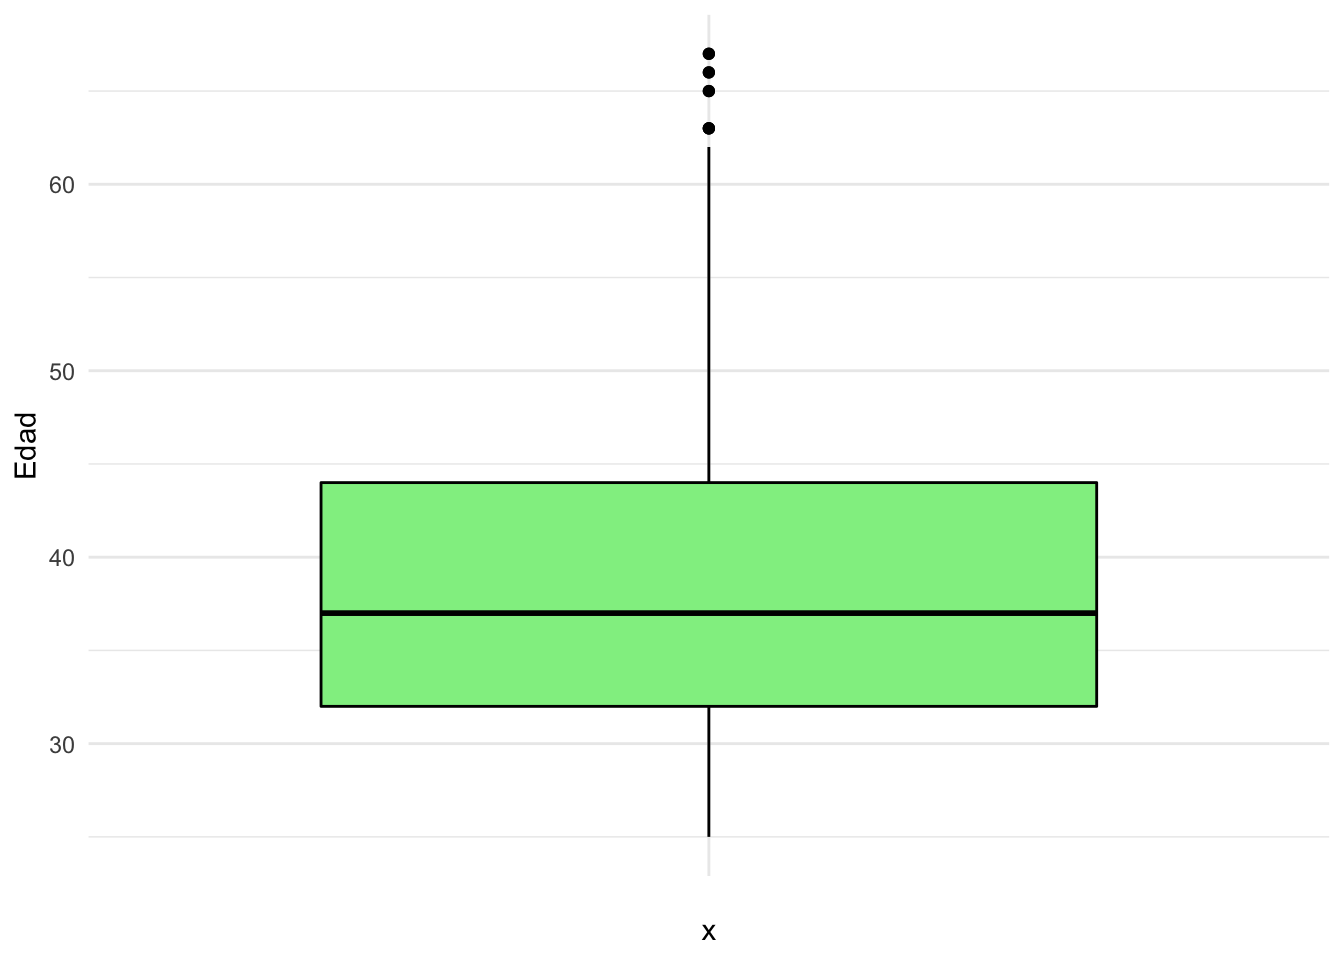
\includegraphics{segundo_trabajo_files/figure-latex/C_1-1.pdf}

\begin{Shaded}
\begin{Highlighting}[]
\FunctionTok{boxplot.stats}\NormalTok{(rh\_data}\SpecialCharTok{$}\NormalTok{Edad)}\SpecialCharTok{$}\NormalTok{out}
\end{Highlighting}
\end{Shaded}

\begin{verbatim}
## [1] 63 66 67 63 65 67 66 65 63
\end{verbatim}

\begin{Shaded}
\begin{Highlighting}[]
\CommentTok{\#Ratio de Pago}
\FunctionTok{ggplot}\NormalTok{(}\AttributeTok{data=}\NormalTok{ rh\_data, }\FunctionTok{aes}\NormalTok{(}\AttributeTok{x=} \StringTok{""}\NormalTok{, }\AttributeTok{y=}\NormalTok{Ratio\_Pago))}\SpecialCharTok{+}\FunctionTok{geom\_boxplot}\NormalTok{(}\AttributeTok{color=}\StringTok{"black"}\NormalTok{,}\AttributeTok{fill=} \StringTok{"lightgreen"}\NormalTok{) }\SpecialCharTok{+} 
\FunctionTok{theme\_minimal}\NormalTok{()}
\end{Highlighting}
\end{Shaded}

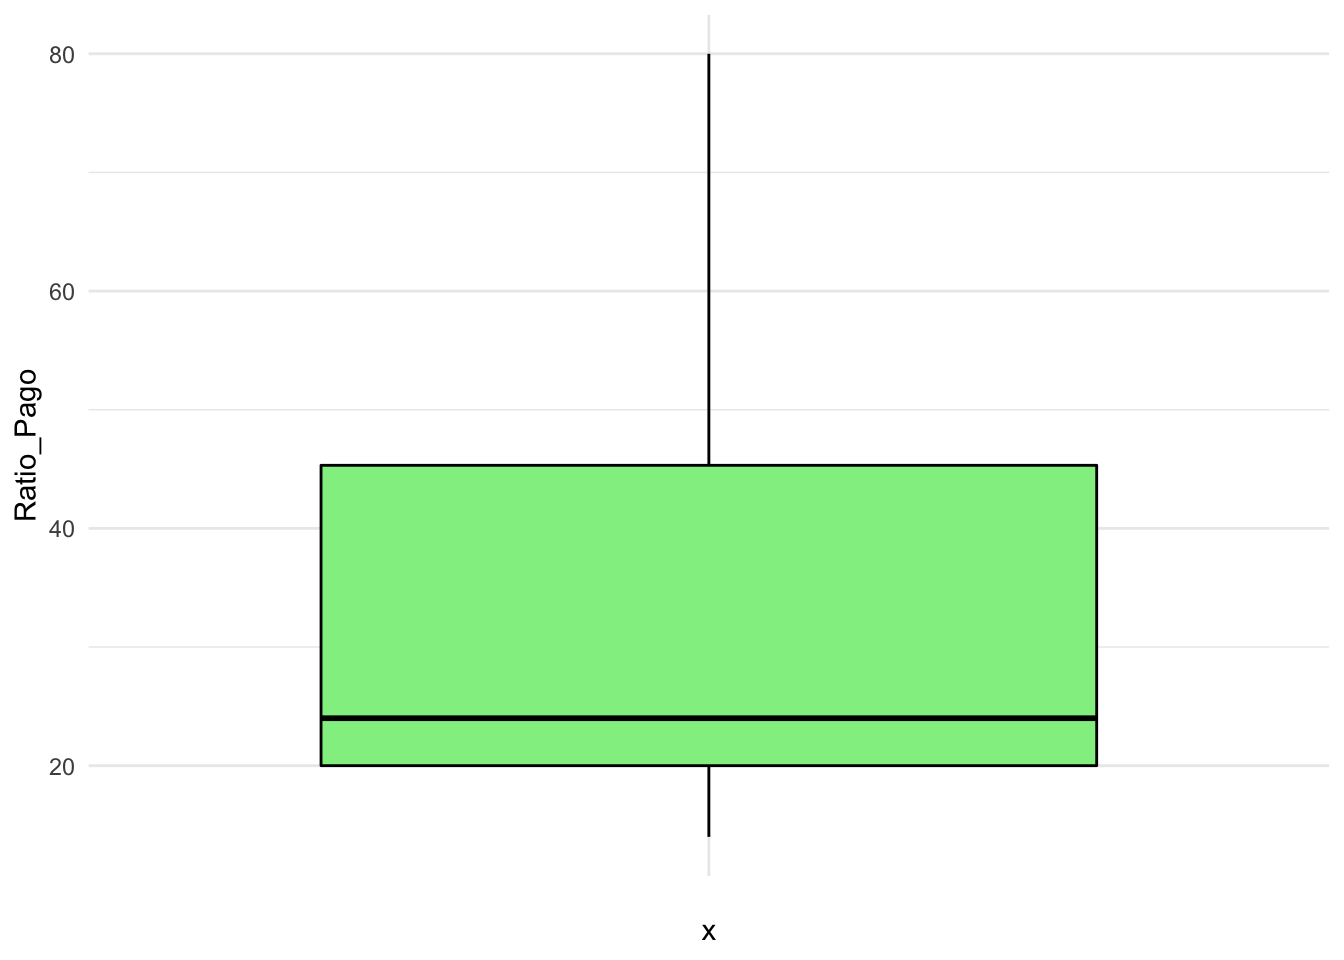
\includegraphics{segundo_trabajo_files/figure-latex/C_1-2.pdf}

\begin{Shaded}
\begin{Highlighting}[]
\FunctionTok{boxplot.stats}\NormalTok{(rh\_data}\SpecialCharTok{$}\NormalTok{Ratio\_Pago)}\SpecialCharTok{$}\NormalTok{out}
\end{Highlighting}
\end{Shaded}

\begin{verbatim}
## numeric(0)
\end{verbatim}

\begin{Shaded}
\begin{Highlighting}[]
\CommentTok{\#Salario}
\FunctionTok{ggplot}\NormalTok{(}\AttributeTok{data=}\NormalTok{ rh\_data, }\FunctionTok{aes}\NormalTok{(}\AttributeTok{x=} \StringTok{""}\NormalTok{,}\AttributeTok{y=}\NormalTok{ Salario)) }\SpecialCharTok{+} \FunctionTok{geom\_boxplot}\NormalTok{(}\AttributeTok{color=}\StringTok{"black"}\NormalTok{,}\AttributeTok{fill=} \StringTok{"lightgreen"}\NormalTok{) }\SpecialCharTok{+} 
\FunctionTok{theme\_minimal}\NormalTok{()}
\end{Highlighting}
\end{Shaded}

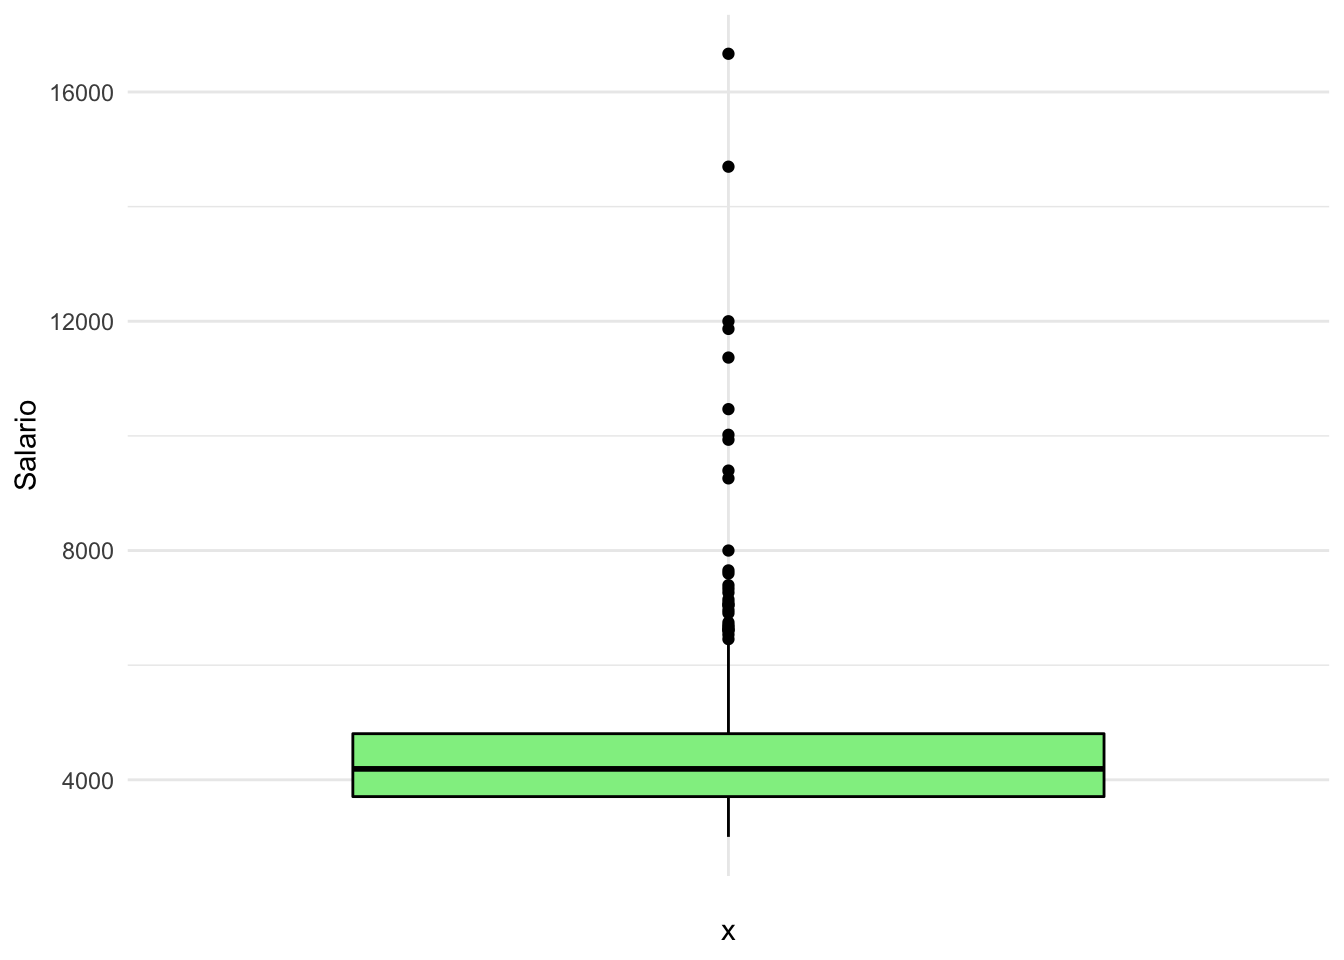
\includegraphics{segundo_trabajo_files/figure-latex/C_1-3.pdf}

\begin{Shaded}
\begin{Highlighting}[]
\FunctionTok{boxplot.stats}\NormalTok{(rh\_data}\SpecialCharTok{$}\NormalTok{Salario)}\SpecialCharTok{$}\NormalTok{out}
\end{Highlighting}
\end{Shaded}

\begin{verbatim}
##  [1]  6962.467  7333.333  6907.533  7091.133  6668.733  7395.267 11366.667
##  [8]  6746.600  9259.200  6618.667 11866.667  6623.400  7653.333  6601.333
## [15]  6533.267 12000.000  7046.667 16666.667  7045.867 10466.667  7265.800
## [22]  8000.000 10019.333  9394.667  9933.267  6694.400  7599.933  7148.400
## [29] 14696.667
\end{verbatim}

\begin{Shaded}
\begin{Highlighting}[]
\CommentTok{\#Dias Trabajados}
\FunctionTok{ggplot}\NormalTok{(}\AttributeTok{data=}\NormalTok{ rh\_data, }\FunctionTok{aes}\NormalTok{(}\AttributeTok{x=} \StringTok{""}\NormalTok{,}\AttributeTok{y=}\NormalTok{ Dias\_Trabajados)) }\SpecialCharTok{+} \FunctionTok{geom\_boxplot}\NormalTok{(}\AttributeTok{color=}\StringTok{"black"}\NormalTok{,}\AttributeTok{fill=} \StringTok{"lightgreen"}\NormalTok{) }\SpecialCharTok{+} 
\FunctionTok{theme\_minimal}\NormalTok{()}
\end{Highlighting}
\end{Shaded}

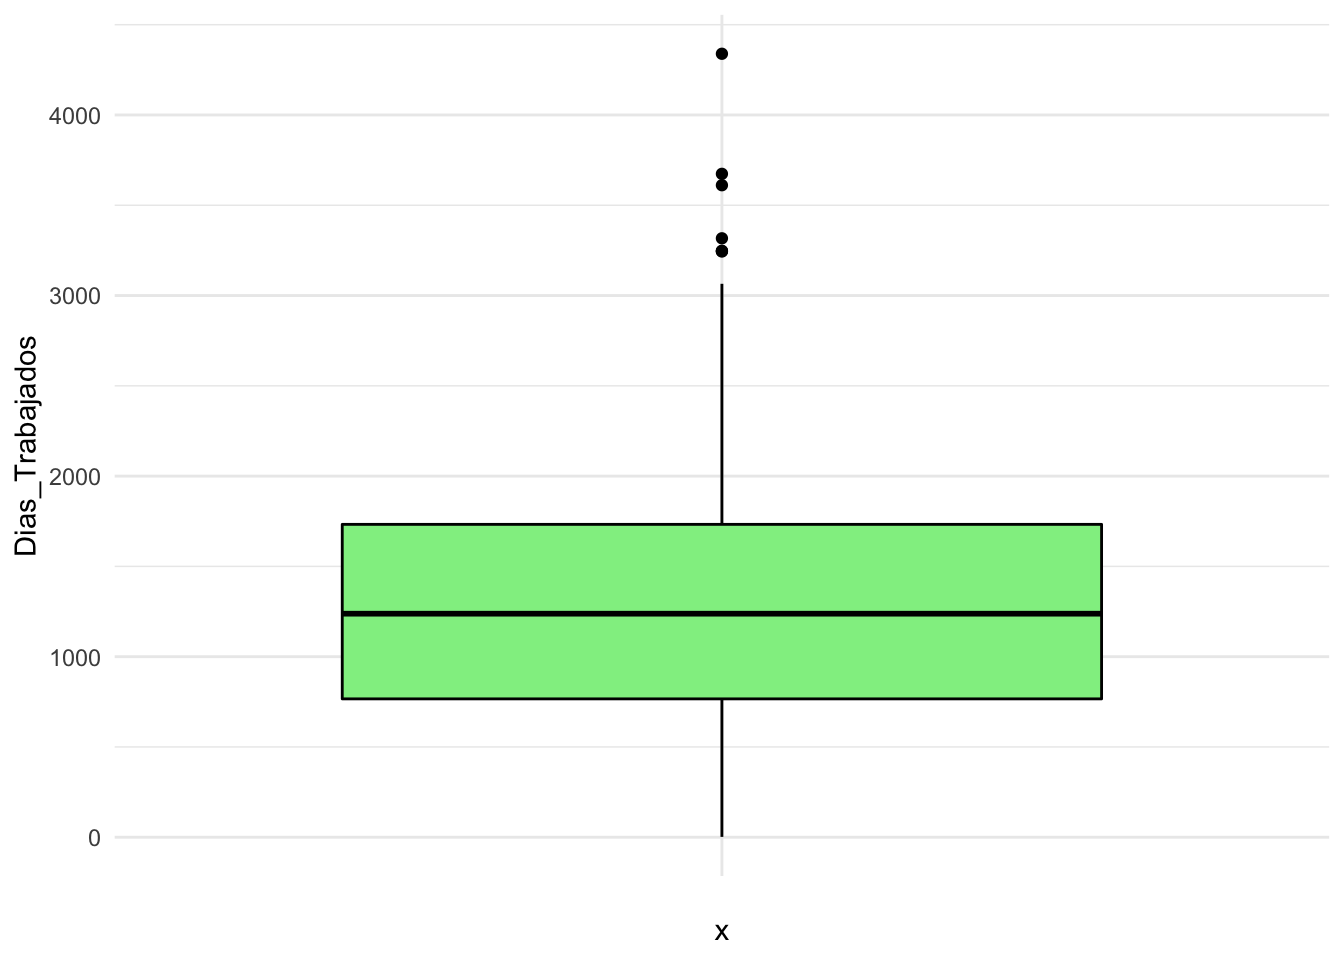
\includegraphics{segundo_trabajo_files/figure-latex/C_1-4.pdf}

\begin{Shaded}
\begin{Highlighting}[]
\FunctionTok{boxplot.stats}\NormalTok{(rh\_data}\SpecialCharTok{$}\NormalTok{Dias\_Trabajados)}\SpecialCharTok{$}\NormalTok{out}
\end{Highlighting}
\end{Shaded}

\begin{verbatim}
## [1] 3317 3247 3247 3244 3611 3674 4339
\end{verbatim}

\begin{Shaded}
\begin{Highlighting}[]
\CommentTok{\#Ausencias}
\FunctionTok{ggplot}\NormalTok{(}\AttributeTok{data=}\NormalTok{ rh\_data, }\FunctionTok{aes}\NormalTok{(}\AttributeTok{x=} \StringTok{""}\NormalTok{,}\AttributeTok{y=}\NormalTok{ Ausencias)) }\SpecialCharTok{+} \FunctionTok{geom\_boxplot}\NormalTok{(}\AttributeTok{color=}\StringTok{"black"}\NormalTok{,}\AttributeTok{fill=} \StringTok{"lightgreen"}\NormalTok{) }\SpecialCharTok{+} 
\FunctionTok{theme\_minimal}\NormalTok{()}
\end{Highlighting}
\end{Shaded}

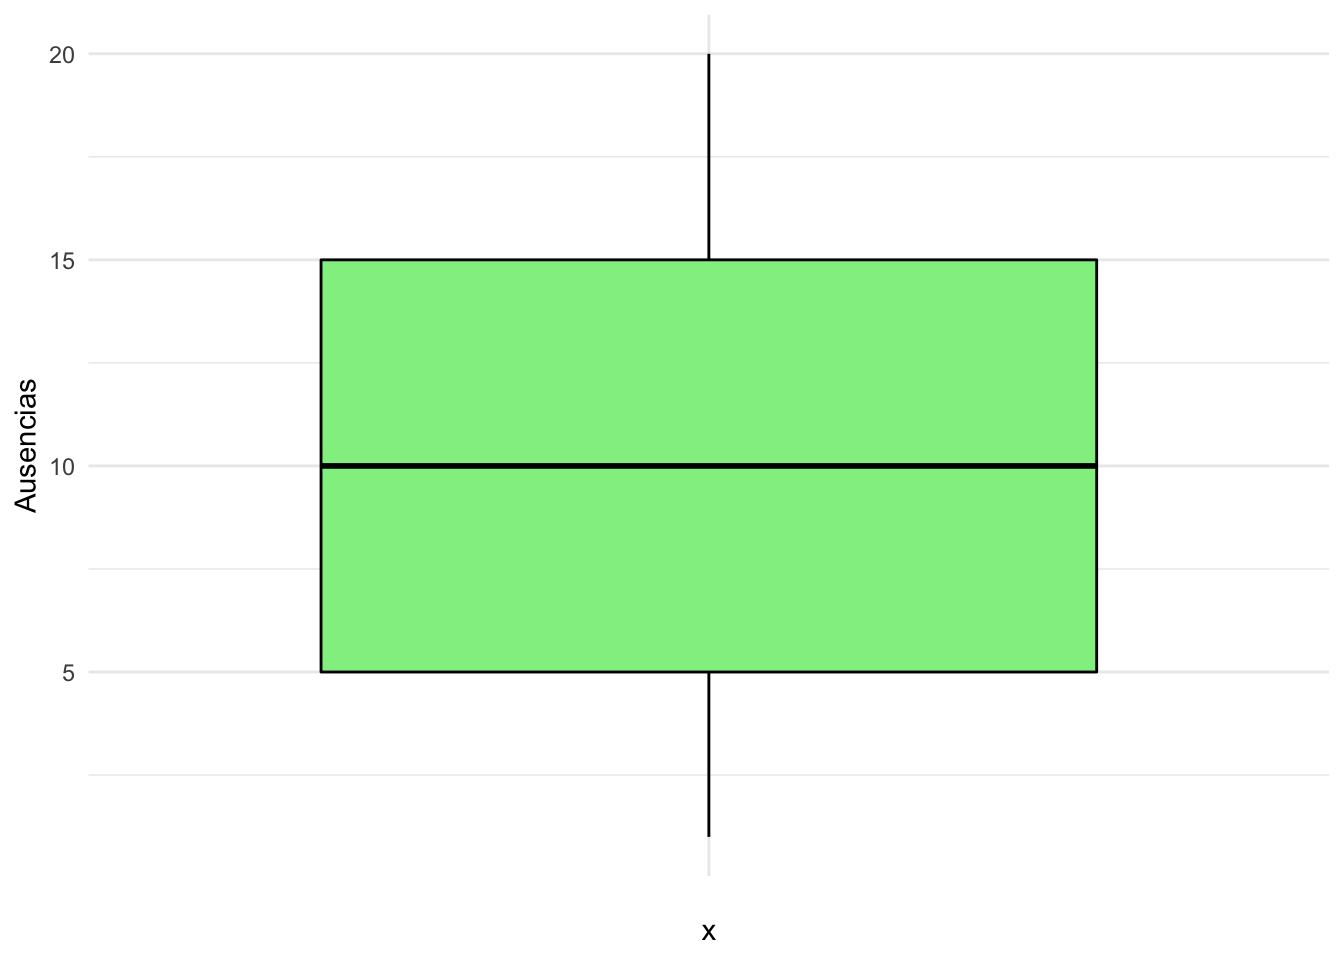
\includegraphics{segundo_trabajo_files/figure-latex/C_1-5.pdf}

\begin{Shaded}
\begin{Highlighting}[]
\FunctionTok{boxplot.stats}\NormalTok{(rh\_data}\SpecialCharTok{$}\NormalTok{Ausencias)}\SpecialCharTok{$}\NormalTok{out}
\end{Highlighting}
\end{Shaded}

\begin{verbatim}
## integer(0)
\end{verbatim}

\textbf{Respuesta:}

\begin{verbatim}
Si bien las variables de "Dias Trabajados", "Salario" y "Edad", poseen datos outlier estos son valores completamente coherentes con el tipo de variable, por lo que no se hace ningún cambio a estos outliers encontrados.
\end{verbatim}

\begin{center}\rule{0.5\linewidth}{0.5pt}\end{center}

\hypertarget{c-realice-anuxe1lisis-de-cuxf3mo-se-relacionan-las-variables-continuas-con-la-variable-de-interuxe9s.-acompauxf1e-con-gruxe1ficos-y-estaduxedsticas.-quuxe9-variables-pudieran-resultar-significativas-a-la-hora-de-modelar-la-probabilidad-de-que-el-trabajador-sea-desvinculado-a-la-empresa}{%
\subsubsection{C) Realice análisis de cómo se relacionan las variables
continuas con la variable de interés. Acompañe con gráficos y
estadísticas. ¿Qué variables pudieran resultar significativas a la hora
de modelar la probabilidad de que el trabajador sea desvinculado a la
empresa?}\label{c-realice-anuxe1lisis-de-cuxf3mo-se-relacionan-las-variables-continuas-con-la-variable-de-interuxe9s.-acompauxf1e-con-gruxe1ficos-y-estaduxedsticas.-quuxe9-variables-pudieran-resultar-significativas-a-la-hora-de-modelar-la-probabilidad-de-que-el-trabajador-sea-desvinculado-a-la-empresa}}

\begin{Shaded}
\begin{Highlighting}[]
\NormalTok{ggpubr}\SpecialCharTok{::}\FunctionTok{ggboxplot}\NormalTok{(rh\_data, }\AttributeTok{y =}\StringTok{"Edad"}\NormalTok{, }\AttributeTok{x=}\StringTok{"Estado"}\NormalTok{, }\AttributeTok{fill =} \StringTok{"Estado"}\NormalTok{)}\SpecialCharTok{+}  
  \FunctionTok{xlab}\NormalTok{(}\StringTok{""}\NormalTok{)}\SpecialCharTok{+} \FunctionTok{ylab}\NormalTok{(}\StringTok{"Edad"}\NormalTok{)}\SpecialCharTok{+}
  \FunctionTok{ggtitle}\NormalTok{(}\StringTok{"Estado Actual de Trabajadores de la Empresa según la Edad"}\NormalTok{)}\SpecialCharTok{+} \FunctionTok{theme\_minimal}\NormalTok{()}
\end{Highlighting}
\end{Shaded}

\includegraphics{segundo_trabajo_files/figure-latex/c1-1.pdf}

\textbf{Respuesta:}

\begin{verbatim}
Se puede apreciar que cuando el valor correspondiente a la edad aumenta, puede encontrarse una mayor probabildad de ser desvinculado.
\end{verbatim}

\begin{Shaded}
\begin{Highlighting}[]
\FunctionTok{anova}\NormalTok{(}\FunctionTok{aov}\NormalTok{(Edad}\SpecialCharTok{\textasciitilde{}}\NormalTok{Estado, }\AttributeTok{data=}\NormalTok{rh\_data)) }
\end{Highlighting}
\end{Shaded}

\begin{verbatim}
## Analysis of Variance Table
## 
## Response: Edad
##            Df Sum Sq Mean Sq F value  Pr(>F)  
## Estado      1    272 271.984  3.4435 0.06446 .
## Residuals 308  24328  78.986                  
## ---
## Signif. codes:  0 '***' 0.001 '**' 0.01 '*' 0.05 '.' 0.1 ' ' 1
\end{verbatim}

\textbf{Respuesta:}

\begin{verbatim}
  La diferencia entre los grupos no seria muy significativa
\end{verbatim}

\hypertarget{variable-de-interuxe9s-estado-y-ratio_pago}{%
\paragraph{Variable de interés Estado y
Ratio\_Pago}\label{variable-de-interuxe9s-estado-y-ratio_pago}}

\begin{Shaded}
\begin{Highlighting}[]
\NormalTok{ggpubr}\SpecialCharTok{::}\FunctionTok{ggboxplot}\NormalTok{(rh\_data, }\AttributeTok{y =}\StringTok{"Ratio\_Pago"}\NormalTok{, }\AttributeTok{x=}\StringTok{"Estado"}\NormalTok{, }\AttributeTok{fill =} \StringTok{"Estado"}\NormalTok{)}\SpecialCharTok{+}  
  \FunctionTok{xlab}\NormalTok{(}\StringTok{""}\NormalTok{)}\SpecialCharTok{+} \FunctionTok{ylab}\NormalTok{(}\StringTok{"Medida de pago por hora"}\NormalTok{)}\SpecialCharTok{+}
  \FunctionTok{ggtitle}\NormalTok{(}\StringTok{"Estado Actual de Trabajadores de la Empresa según el Ratio de Pago"}\NormalTok{)}\SpecialCharTok{+} \FunctionTok{theme\_minimal}\NormalTok{()}
\end{Highlighting}
\end{Shaded}

\includegraphics{segundo_trabajo_files/figure-latex/c2-1-1.pdf}
\textbf{Respuesta}

\begin{verbatim}
Pareciera que a mayor Ratio de Pago, mas probable es que el trabajador se encuentre   vinculado (0) a la empresa.
\end{verbatim}

\begin{Shaded}
\begin{Highlighting}[]
\FunctionTok{anova}\NormalTok{(}\FunctionTok{aov}\NormalTok{(Ratio\_Pago}\SpecialCharTok{\textasciitilde{}}\NormalTok{Estado, }\AttributeTok{data=}\NormalTok{rh\_data)) }
\end{Highlighting}
\end{Shaded}

\begin{verbatim}
## Analysis of Variance Table
## 
## Response: Ratio_Pago
##            Df Sum Sq Mean Sq F value    Pr(>F)    
## Estado      1   2907 2907.12  12.751 0.0004126 ***
## Residuals 308  70219  227.99                      
## ---
## Signif. codes:  0 '***' 0.001 '**' 0.01 '*' 0.05 '.' 0.1 ' ' 1
\end{verbatim}

\textbf{Respuesta:}

\begin{verbatim}
La diferencia entre los grupos seria muy significativa
\end{verbatim}

\hypertarget{variable-de-interuxe9s-estado-y-salario}{%
\subparagraph{Variable de interés Estado y
Salario}\label{variable-de-interuxe9s-estado-y-salario}}

\begin{Shaded}
\begin{Highlighting}[]
\NormalTok{ggpubr}\SpecialCharTok{::}\FunctionTok{ggboxplot}\NormalTok{(rh\_data, }\AttributeTok{y =}\StringTok{"Salario"}\NormalTok{, }\AttributeTok{x=}\StringTok{"Estado"}\NormalTok{, }\AttributeTok{fill =} \StringTok{"Estado"}\NormalTok{)}\SpecialCharTok{+}  
  \FunctionTok{xlab}\NormalTok{(}\StringTok{""}\NormalTok{)}\SpecialCharTok{+} \FunctionTok{ylab}\NormalTok{(}\StringTok{"Salario Mensual (USD)"}\NormalTok{)}\SpecialCharTok{+}
  \FunctionTok{ggtitle}\NormalTok{(}\StringTok{"Estado Actual de Trabajadores de la Empresa según el Salario Mensual"}\NormalTok{)}\SpecialCharTok{+} \FunctionTok{theme\_minimal}\NormalTok{()}
\end{Highlighting}
\end{Shaded}

\includegraphics{segundo_trabajo_files/figure-latex/c_3-1.pdf}
\textbf{Respuesta:}

\begin{verbatim}
No pareciera que exista mucha diferencia entre los vinculados y desvinculados según el Salario
\end{verbatim}

\begin{Shaded}
\begin{Highlighting}[]
\FunctionTok{anova}\NormalTok{(}\FunctionTok{aov}\NormalTok{(Salario}\SpecialCharTok{\textasciitilde{}}\NormalTok{Estado, }\AttributeTok{data=}\NormalTok{rh\_data)) }
\end{Highlighting}
\end{Shaded}

\begin{verbatim}
## Analysis of Variance Table
## 
## Response: Salario
##            Df    Sum Sq Mean Sq F value Pr(>F)
## Estado      1     61134   61134  0.0217 0.8831
## Residuals 308 869311482 2822440
\end{verbatim}

\textbf{Respuesta:}

\begin{verbatim}
La diferencia entre los grupos No seria significativa
\end{verbatim}

\hypertarget{variable-de-interuxe9s-estado-y-duxedas-trabajados}{%
\subparagraph{Variable de interés Estado y Días
Trabajados}\label{variable-de-interuxe9s-estado-y-duxedas-trabajados}}

\begin{Shaded}
\begin{Highlighting}[]
\NormalTok{ggpubr}\SpecialCharTok{::}\FunctionTok{ggboxplot}\NormalTok{(rh\_data, }\AttributeTok{y =}\StringTok{"Dias\_Trabajados"}\NormalTok{, }\AttributeTok{x=}\StringTok{"Estado"}\NormalTok{, }\AttributeTok{fill =} \StringTok{"Estado"}\NormalTok{)}\SpecialCharTok{+}  
  \FunctionTok{xlab}\NormalTok{(}\StringTok{""}\NormalTok{)}\SpecialCharTok{+} \FunctionTok{ylab}\NormalTok{(}\StringTok{"Días que lleva o llevaba trabajando en la empresa"}\NormalTok{)}\SpecialCharTok{+}
  \FunctionTok{ggtitle}\NormalTok{(}\StringTok{"Estado Actual de Trabajadores de la Empresa según Días que lleva trabajando"}\NormalTok{)}\SpecialCharTok{+} 
  \FunctionTok{theme\_minimal}\NormalTok{()}
\end{Highlighting}
\end{Shaded}

\includegraphics{segundo_trabajo_files/figure-latex/c_4-1.pdf}
\textbf{Respuesta:}

\begin{verbatim}
Pareciera que a mayor cantidad de días trabajados que lleva un empleado, mas probable es que el trabajador se encuentre vinculado(0) a la empresa.
\end{verbatim}

\begin{Shaded}
\begin{Highlighting}[]
\FunctionTok{anova}\NormalTok{(}\FunctionTok{aov}\NormalTok{(Dias\_Trabajados}\SpecialCharTok{\textasciitilde{}}\NormalTok{Estado, }\AttributeTok{data=}\NormalTok{rh\_data)) }
\end{Highlighting}
\end{Shaded}

\begin{verbatim}
## Analysis of Variance Table
## 
## Response: Dias_Trabajados
##            Df    Sum Sq  Mean Sq F value    Pr(>F)    
## Estado      1  44824671 44824671  99.942 < 2.2e-16 ***
## Residuals 308 138139478   448505                      
## ---
## Signif. codes:  0 '***' 0.001 '**' 0.01 '*' 0.05 '.' 0.1 ' ' 1
\end{verbatim}

\textbf{Respuesta:}

\begin{verbatim}
La diferencia entre los grupos seria muy significativa
\end{verbatim}

\hypertarget{variable-de-interuxe9s-estado-y-ausencias}{%
\subparagraph{Variable de interés Estado y
Ausencias}\label{variable-de-interuxe9s-estado-y-ausencias}}

\begin{Shaded}
\begin{Highlighting}[]
\NormalTok{ggpubr}\SpecialCharTok{::}\FunctionTok{ggboxplot}\NormalTok{(rh\_data, }\AttributeTok{y =}\StringTok{"Ausencias"}\NormalTok{, }\AttributeTok{x=}\StringTok{"Estado"}\NormalTok{, }\AttributeTok{fill =} \StringTok{"Estado"}\NormalTok{)}\SpecialCharTok{+}  
  \FunctionTok{xlab}\NormalTok{(}\StringTok{""}\NormalTok{)}\SpecialCharTok{+} \FunctionTok{ylab}\NormalTok{(}\StringTok{"Días que ha faltado a trabajar"}\NormalTok{)}\SpecialCharTok{+}
  \FunctionTok{ggtitle}\NormalTok{(}\StringTok{"Estado Actual de Trabajadores de la Empresa según Días que ha faltado"}\NormalTok{)}\SpecialCharTok{+} 
  \FunctionTok{theme\_minimal}\NormalTok{()}
\end{Highlighting}
\end{Shaded}

\includegraphics{segundo_trabajo_files/figure-latex/c_5-1.pdf}
\textbf{Respuesta:}

\begin{verbatim}
No pareciera que exista mucha diferencia entre los vinculados y desvinculados según la cantidad de días que han faltado al Trabajo.
\end{verbatim}

\begin{Shaded}
\begin{Highlighting}[]
\FunctionTok{anova}\NormalTok{(}\FunctionTok{aov}\NormalTok{(Ausencias}\SpecialCharTok{\textasciitilde{}}\NormalTok{Estado, }\AttributeTok{data=}\NormalTok{rh\_data)) }
\end{Highlighting}
\end{Shaded}

\begin{verbatim}
## Analysis of Variance Table
## 
## Response: Ausencias
##            Df  Sum Sq Mean Sq F value Pr(>F)
## Estado      1     0.4   0.390  0.0114 0.9151
## Residuals 308 10549.9  34.253
\end{verbatim}

\textbf{Respuesta:} La diferencia entre los grupos No seria muy
significativa

\begin{center}\rule{0.5\linewidth}{0.5pt}\end{center}

\hypertarget{d-como-se-relacionan-las-variables-categuxf3ricas-con-la-variable-de-interuxe9s}{%
\subsubsection{D) Como se relacionan las variables categóricas con la
variable de
interés}\label{d-como-se-relacionan-las-variables-categuxf3ricas-con-la-variable-de-interuxe9s}}

\hypertarget{se-realiza-un-test-ux3c72-de-dependencia-ademuxe1s-de-mostrar-distribuciuxf3n-de-las-frecuencias-con-tablas-de-contingencia.}{%
\paragraph{Se Realiza un test χ2 de dependencia, además de mostrar
distribución de las frecuencias con tablas de
contingencia.}\label{se-realiza-un-test-ux3c72-de-dependencia-ademuxe1s-de-mostrar-distribuciuxf3n-de-las-frecuencias-con-tablas-de-contingencia.}}

\hypertarget{variable-de-interuxe9s-estado-y-sexo}{%
\paragraph{Variable de interés Estado y
Sexo}\label{variable-de-interuxe9s-estado-y-sexo}}

\begin{Shaded}
\begin{Highlighting}[]
\FunctionTok{prop.table}\NormalTok{(}\FunctionTok{table}\NormalTok{(rh\_data}\SpecialCharTok{$}\NormalTok{Estado, rh\_data}\SpecialCharTok{$}\NormalTok{Sexo), }\DecValTok{2}\NormalTok{)}
\end{Highlighting}
\end{Shaded}

\begin{verbatim}
##    
##        Female      Male
##   0 0.5706215 0.6165414
##   1 0.4293785 0.3834586
\end{verbatim}

\begin{Shaded}
\begin{Highlighting}[]
\FunctionTok{mosaicplot}\NormalTok{(}\SpecialCharTok{\textasciitilde{}}\NormalTok{Sexo}\SpecialCharTok{+}\NormalTok{Estado, }\AttributeTok{data=}\NormalTok{rh\_data, }\AttributeTok{main =} \StringTok{"Distribución de los datos basados en estado y sexo"}\NormalTok{, }\AttributeTok{shade=}\NormalTok{F)}
\end{Highlighting}
\end{Shaded}

\includegraphics{segundo_trabajo_files/figure-latex/d_1-1.pdf}

\hypertarget{test}{%
\subparagraph{Test}\label{test}}

\begin{Shaded}
\begin{Highlighting}[]
\FunctionTok{chisq.test}\NormalTok{(rh\_data}\SpecialCharTok{$}\NormalTok{Sexo, rh\_data}\SpecialCharTok{$}\NormalTok{Estado)}
\end{Highlighting}
\end{Shaded}

\begin{verbatim}
## 
##  Pearson's Chi-squared test with Yates' continuity correction
## 
## data:  rh_data$Sexo and rh_data$Estado
## X-squared = 0.48585, df = 1, p-value = 0.4858
\end{verbatim}

\textbf{Respuesta:}

\begin{verbatim}
No existe relación entre las variables, ya que se acepta la independencia entre ellas. Considerando un 95% de confianza. No se espera que sea una variable significativa.
\end{verbatim}

\hypertarget{variable-de-interuxe9s-estado-y-estado_civil}{%
\paragraph{Variable de interés Estado y
Estado\_Civil}\label{variable-de-interuxe9s-estado-y-estado_civil}}

\begin{Shaded}
\begin{Highlighting}[]
\FunctionTok{prop.table}\NormalTok{(}\FunctionTok{table}\NormalTok{(rh\_data}\SpecialCharTok{$}\NormalTok{Estado, rh\_data}\SpecialCharTok{$}\NormalTok{Estado\_Civil), }\DecValTok{2}\NormalTok{)}
\end{Highlighting}
\end{Shaded}

\begin{verbatim}
##    
##             1         2         3         4         5
##   0 0.4666667 0.5284553 0.6666667 0.6715328 0.5000000
##   1 0.5333333 0.4715447 0.3333333 0.3284672 0.5000000
\end{verbatim}

\begin{Shaded}
\begin{Highlighting}[]
\FunctionTok{mosaicplot}\NormalTok{(}\SpecialCharTok{\textasciitilde{}}\NormalTok{Estado\_Civil}\SpecialCharTok{+}\NormalTok{Estado, }\AttributeTok{data=}\NormalTok{rh\_data, }\AttributeTok{main =} \StringTok{"Distribución de los datos basados en estado y estado civil"}\NormalTok{, }\AttributeTok{shade=}\NormalTok{F)}
\end{Highlighting}
\end{Shaded}

\includegraphics{segundo_trabajo_files/figure-latex/d_2-1.pdf}

\#\#\#\#\#Test

\begin{Shaded}
\begin{Highlighting}[]
\FunctionTok{chisq.test}\NormalTok{(rh\_data}\SpecialCharTok{$}\NormalTok{Estado\_Civil, rh\_data}\SpecialCharTok{$}\NormalTok{Estado)}
\end{Highlighting}
\end{Shaded}

\begin{verbatim}
## Warning in stats::chisq.test(x, y, ...): Chi-squared approximation may be
## incorrect
\end{verbatim}

\begin{verbatim}
## 
##  Pearson's Chi-squared test
## 
## data:  rh_data$Estado_Civil and rh_data$Estado
## X-squared = 8.1386, df = 4, p-value = 0.08663
\end{verbatim}

\textbf{Respuesta:}

\begin{verbatim}
No existe relación entre las variables, ya que se acepta la independencia entre ellas. considerando un 95% de confianza. No se espera que sea una variable significativa.
\end{verbatim}

\hypertarget{variable-de-interuxe9s-estado-y-departamento}{%
\subparagraph{Variable de interés Estado y
Departamento}\label{variable-de-interuxe9s-estado-y-departamento}}

\begin{Shaded}
\begin{Highlighting}[]
\FunctionTok{prop.table}\NormalTok{(}\FunctionTok{table}\NormalTok{(rh\_data}\SpecialCharTok{$}\NormalTok{Estado, rh\_data}\SpecialCharTok{$}\NormalTok{Departamento), }\DecValTok{2}\NormalTok{)}
\end{Highlighting}
\end{Shaded}

\begin{verbatim}
##    
##     Admin Offices Executive Office     IT/IS Production     Sales
##   0     0.8000000        1.0000000 0.7000000  0.5096154 0.8387097
##   1     0.2000000        0.0000000 0.3000000  0.4903846 0.1612903
##    
##     Software Engineering
##   0            0.7000000
##   1            0.3000000
\end{verbatim}

\begin{Shaded}
\begin{Highlighting}[]
\FunctionTok{mosaicplot}\NormalTok{(}\SpecialCharTok{\textasciitilde{}}\NormalTok{Departamento}\SpecialCharTok{+}\NormalTok{Estado, }\AttributeTok{data=}\NormalTok{rh\_data,  }\AttributeTok{main =} \StringTok{"Distribución de los datos basados en estado y Departamento"}\NormalTok{, }\AttributeTok{shade=}\NormalTok{F)}
\end{Highlighting}
\end{Shaded}

\includegraphics{segundo_trabajo_files/figure-latex/d_3-1.pdf}
\#\#\#\#\#Test

\begin{Shaded}
\begin{Highlighting}[]
\FunctionTok{chisq.test}\NormalTok{(rh\_data}\SpecialCharTok{$}\NormalTok{Departamento, rh\_data}\SpecialCharTok{$}\NormalTok{Estado)}
\end{Highlighting}
\end{Shaded}

\begin{verbatim}
## Warning in stats::chisq.test(x, y, ...): Chi-squared approximation may be
## incorrect
\end{verbatim}

\begin{verbatim}
## 
##  Pearson's Chi-squared test
## 
## data:  rh_data$Departamento and rh_data$Estado
## X-squared = 19.007, df = 5, p-value = 0.001917
\end{verbatim}

\textbf{Respuesta:}

\begin{verbatim}
Existe relación entre las variables,  que se rechaza la independencia entre ellas. considerando un 95% de confianza. Se espera que sea una variable significativa.
\end{verbatim}

\hypertarget{variable-de-interuxe9s-estado-y-posicion}{%
\subparagraph{Variable de interés Estado y
Posicion}\label{variable-de-interuxe9s-estado-y-posicion}}

\begin{Shaded}
\begin{Highlighting}[]
\FunctionTok{prop.table}\NormalTok{(}\FunctionTok{table}\NormalTok{(rh\_data}\SpecialCharTok{$}\NormalTok{Estado,rh\_data}\SpecialCharTok{$}\NormalTok{Posicion), }\DecValTok{2}\NormalTok{)}
\end{Highlighting}
\end{Shaded}

\begin{verbatim}
##    
##     Accountant I Administrative Assistant Area Sales Manager BI Developer
##   0    1.0000000                0.6666667          0.8518519    1.0000000
##   1    0.0000000                0.3333333          0.1481481    0.0000000
##    
##     BI Director       CIO Data Architect Database Administrator
##   0   1.0000000 1.0000000      1.0000000              0.5384615
##   1   0.0000000 0.0000000      0.0000000              0.4615385
##    
##     Director of Operations Director of Sales IT Director IT Manager - DB
##   0              1.0000000         1.0000000   1.0000000       0.5000000
##   1              0.0000000         0.0000000   0.0000000       0.5000000
##    
##     IT Manager - Infra IT Manager - Support IT Support Network Engineer
##   0          1.0000000            1.0000000  1.0000000        0.8888889
##   1          0.0000000            0.0000000  0.0000000        0.1111111
##    
##     President & CEO Production Manager Production Technician I
##   0       1.0000000          0.6428571               0.5367647
##   1       0.0000000          0.3571429               0.4632353
##    
##     Production Technician II Sales Manager Senior BI Developer
##   0                0.4035088     0.6666667           1.0000000
##   1                0.5964912     0.3333333           0.0000000
##    
##     Shared Services Manager Software Engineer Software Engineering Manager
##   0               0.5000000         0.6666667                    1.0000000
##   1               0.5000000         0.3333333                    0.0000000
##    
##     Sr. Accountant   Sr. DBA Sr. Network Engineer
##   0      1.0000000 0.0000000            0.4000000
##   1      0.0000000 1.0000000            0.6000000
\end{verbatim}

\begin{Shaded}
\begin{Highlighting}[]
\FunctionTok{mosaicplot}\NormalTok{(}\SpecialCharTok{\textasciitilde{}}\NormalTok{Posicion}\SpecialCharTok{+}\NormalTok{Estado, }\AttributeTok{data=}\NormalTok{rh\_data, }\AttributeTok{main =} \StringTok{"Distribución de los datos basados en estado y Posición en la empresa"}\NormalTok{, }\AttributeTok{shade=}\NormalTok{F)}
\end{Highlighting}
\end{Shaded}

\includegraphics{segundo_trabajo_files/figure-latex/D_4-1.pdf}

\hypertarget{test-1}{%
\subparagraph{Test}\label{test-1}}

\begin{Shaded}
\begin{Highlighting}[]
\FunctionTok{chisq.test}\NormalTok{(rh\_data}\SpecialCharTok{$}\NormalTok{Posicion, rh\_data}\SpecialCharTok{$}\NormalTok{Estado)}
\end{Highlighting}
\end{Shaded}

\begin{verbatim}
## Warning in stats::chisq.test(x, y, ...): Chi-squared approximation may be
## incorrect
\end{verbatim}

\begin{verbatim}
## 
##  Pearson's Chi-squared test
## 
## data:  rh_data$Posicion and rh_data$Estado
## X-squared = 46.149, df = 27, p-value = 0.01226
\end{verbatim}

\textbf{Respuesta:}

\begin{verbatim}
Existe relación entre las variables, ya que se rechaza la independencia entre ellas. considerando un 95% de confianza. Se espera que sea una variable significativa.
\end{verbatim}

\hypertarget{variable-de-interuxe9s-estado-y-desempeuxf1o}{%
\paragraph{Variable de interés Estado y
Desempeño}\label{variable-de-interuxe9s-estado-y-desempeuxf1o}}

\begin{Shaded}
\begin{Highlighting}[]
\FunctionTok{prop.table}\NormalTok{(}\FunctionTok{table}\NormalTok{(rh\_data}\SpecialCharTok{$}\NormalTok{Estado,rh\_data}\SpecialCharTok{$}\NormalTok{Desempenio), }\DecValTok{2}\NormalTok{)}
\end{Highlighting}
\end{Shaded}

\begin{verbatim}
##    
##     90-day meets   Exceeds Exceptional Fully Meets N/A- too early to review
##   0    0.5161290 0.6428571   1.0000000   0.6243094                0.4054054
##   1    0.4838710 0.3571429   0.0000000   0.3756906                0.5945946
##    
##     Needs Improvement       PIP
##   0         0.4666667 0.5555556
##   1         0.5333333 0.4444444
\end{verbatim}

\begin{Shaded}
\begin{Highlighting}[]
\FunctionTok{mosaicplot}\NormalTok{(}\SpecialCharTok{\textasciitilde{}}\NormalTok{Desempenio}\SpecialCharTok{+}\NormalTok{Estado, }\AttributeTok{data=}\NormalTok{rh\_data, }\AttributeTok{main =} \StringTok{"Distribución de los datos basados en estado y desempeño"}\NormalTok{, }\AttributeTok{shade=}\NormalTok{F)}
\end{Highlighting}
\end{Shaded}

\includegraphics{segundo_trabajo_files/figure-latex/D_5-1.pdf}
\#\#\#\#\# Test

\begin{Shaded}
\begin{Highlighting}[]
\FunctionTok{chisq.test}\NormalTok{(rh\_data}\SpecialCharTok{$}\NormalTok{Desempenio, rh\_data}\SpecialCharTok{$}\NormalTok{Estado)}
\end{Highlighting}
\end{Shaded}

\begin{verbatim}
## Warning in stats::chisq.test(x, y, ...): Chi-squared approximation may be
## incorrect
\end{verbatim}

\begin{verbatim}
## 
##  Pearson's Chi-squared test
## 
## data:  rh_data$Desempenio and rh_data$Estado
## X-squared = 14.36, df = 6, p-value = 0.02586
\end{verbatim}

\textbf{Respuesta:}

\begin{verbatim}
Existe relación entre las variables, ya que se rechaza la independencia entre ellas considerando un 95% de confianza. Se espera que sea una variable significativa.
\end{verbatim}

\begin{center}\rule{0.5\linewidth}{0.5pt}\end{center}

\hypertarget{e-realice-una-separaciuxf3n-de-la-base-de-datos-en-un-set-de-entrenamiento-y-set-de-validaciuxf3n-utilice-una-proporciuxf3n-de-7525-respectivamente.-para-poder-replicar-sus-resultados-fije-una-semilla-antes-de-obtener-los-uxedndices.-para-ello-utilice-la-funciuxf3n-set.seed2021.}{%
\subsection{E) Realice una separación de la base de datos en un set de
entrenamiento y set de validación, utilice una proporción de 75:25
respectivamente. Para poder replicar sus resultados, fije una semilla
antes de obtener los índices. Para ello, utilice la función
set.seed(2021).}\label{e-realice-una-separaciuxf3n-de-la-base-de-datos-en-un-set-de-entrenamiento-y-set-de-validaciuxf3n-utilice-una-proporciuxf3n-de-7525-respectivamente.-para-poder-replicar-sus-resultados-fije-una-semilla-antes-de-obtener-los-uxedndices.-para-ello-utilice-la-funciuxf3n-set.seed2021.}}

\begin{Shaded}
\begin{Highlighting}[]
\FunctionTok{set.seed}\NormalTok{(}\DecValTok{2021}\NormalTok{)}
\CommentTok{\#listado de muestras a tomar}
\NormalTok{sampling }\OtherTok{\textless{}{-}} \FunctionTok{sample}\NormalTok{(}\DecValTok{1}\SpecialCharTok{:}\FunctionTok{nrow}\NormalTok{(rh\_data), }\AttributeTok{size =} \FloatTok{0.75}\SpecialCharTok{*}\FunctionTok{nrow}\NormalTok{(rh\_data), }\AttributeTok{replace =} \ConstantTok{FALSE}\NormalTok{) }
\NormalTok{modelo\_train }\OtherTok{\textless{}{-}}\NormalTok{ rh\_data }\SpecialCharTok{\%\textgreater{}\%} \FunctionTok{slice}\NormalTok{(sampling) }\CommentTok{\#data de entrenamiento}
\NormalTok{modelo\_test }\OtherTok{\textless{}{-}}\NormalTok{ rh\_data }\SpecialCharTok{\%\textgreater{}\%} \FunctionTok{slice}\NormalTok{(}\SpecialCharTok{{-}}\NormalTok{sampling) }\CommentTok{\#data de validación}
\end{Highlighting}
\end{Shaded}

\hypertarget{f-con-los-datos-de-entrenamiento-ajuste-un-modelo-de-regresiuxf3n-loguxedstica-para-estudiar-la-probabilidad-de-que-el-trabajador-sea-desvinculado-de-la-empresa.-para-ello-utilice-las-variables-edad-y-desempeuxf1o.}{%
\subsection{F) Con los datos de entrenamiento ajuste un modelo de
regresión logística para estudiar la probabilidad de que el trabajador
sea desvinculado de la empresa. Para ello, utilice las variables edad y
desempeño.}\label{f-con-los-datos-de-entrenamiento-ajuste-un-modelo-de-regresiuxf3n-loguxedstica-para-estudiar-la-probabilidad-de-que-el-trabajador-sea-desvinculado-de-la-empresa.-para-ello-utilice-las-variables-edad-y-desempeuxf1o.}}

\begin{Shaded}
\begin{Highlighting}[]
\NormalTok{modelo\_desvinculacion }\OtherTok{\textless{}{-}} \FunctionTok{glm}\NormalTok{(Estado }\SpecialCharTok{\textasciitilde{}}\NormalTok{ Edad }\SpecialCharTok{+}\NormalTok{ Desempenio, }
                             \AttributeTok{data =}\NormalTok{ modelo\_train,}
                             \AttributeTok{family =} \FunctionTok{binomial}\NormalTok{(}\AttributeTok{link =} \StringTok{"logit"}\NormalTok{))}
\FunctionTok{summary}\NormalTok{(modelo\_desvinculacion)}
\end{Highlighting}
\end{Shaded}

\begin{verbatim}
## 
## Call:
## glm(formula = Estado ~ Edad + Desempenio, family = binomial(link = "logit"), 
##     data = modelo_train)
## 
## Deviance Residuals: 
##     Min       1Q   Median       3Q      Max  
## -1.6754  -0.9672  -0.7688   1.1903   1.8741  
## 
## Coefficients:
##                                      Estimate Std. Error z value Pr(>|z|)   
## (Intercept)                          -1.73355    0.74664  -2.322  0.02024 * 
## Edad                                  0.05007    0.01647   3.039  0.00237 **
## DesempenioExceeds                    -1.38505    0.68098  -2.034  0.04196 * 
## DesempenioExceptional               -16.78511 1058.55891  -0.016  0.98735   
## DesempenioFully Meets                -0.78597    0.45760  -1.718  0.08587 . 
## DesempenioN/A- too early to review    0.40178    0.56572   0.710  0.47757   
## DesempenioNeeds Improvement          -0.22693    0.74007  -0.307  0.75913   
## DesempenioPIP                        -0.41360    0.88193  -0.469  0.63909   
## ---
## Signif. codes:  0 '***' 0.001 '**' 0.01 '*' 0.05 '.' 0.1 ' ' 1
## 
## (Dispersion parameter for binomial family taken to be 1)
## 
##     Null deviance: 313.97  on 231  degrees of freedom
## Residual deviance: 290.26  on 224  degrees of freedom
## AIC: 306.26
## 
## Number of Fisher Scoring iterations: 15
\end{verbatim}

\hypertarget{g-calcule-e-interprete-los-or-correspondientes-al-modelo}{%
\subsection{G) Calcule e interprete los OR correspondientes al
modelo,}\label{g-calcule-e-interprete-los-or-correspondientes-al-modelo}}

\hypertarget{son-estos-factores-protectores-o-agravantes-de-la-desvinculaciuxf3n-del-trabajador}{%
\subsection{¿son estos factores protectores o agravantes de la
desvinculación del
trabajador?}\label{son-estos-factores-protectores-o-agravantes-de-la-desvinculaciuxf3n-del-trabajador}}

\begin{Shaded}
\begin{Highlighting}[]
\NormalTok{broom}\SpecialCharTok{::}\FunctionTok{tidy}\NormalTok{(modelo\_desvinculacion) }\SpecialCharTok{\%\textgreater{}\%} \FunctionTok{mutate}\NormalTok{(}\AttributeTok{OR  =} \FunctionTok{exp}\NormalTok{(estimate))}
\end{Highlighting}
\end{Shaded}

\begin{verbatim}
## # A tibble: 8 x 6
##   term                          estimate std.error statistic p.value          OR
##   <chr>                            <dbl>     <dbl>     <dbl>   <dbl>       <dbl>
## 1 (Intercept)                    -1.73      0.747    -2.32   0.0202      1.77e-1
## 2 Edad                            0.0501    0.0165    3.04   0.00237     1.05e+0
## 3 DesempenioExceeds              -1.39      0.681    -2.03   0.0420      2.50e-1
## 4 DesempenioExceptional         -16.8    1059.       -0.0159 0.987       5.13e-8
## 5 DesempenioFully Meets          -0.786     0.458    -1.72   0.0859      4.56e-1
## 6 DesempenioN/A- too early to ~   0.402     0.566     0.710  0.478       1.49e+0
## 7 DesempenioNeeds Improvement    -0.227     0.740    -0.307  0.759       7.97e-1
## 8 DesempenioPIP                  -0.414     0.882    -0.469  0.639       6.61e-1
\end{verbatim}

\textbf{Respuesta:}

\begin{verbatim}
Edad ~ A medida que aumenta la edad promedio del trabajador, mayor probabilidad de que este sea desvinculado.(aumento del 5%)

DesempenioExceeds ~ La probabilidad de desvinculación de un trabajador es menor si su desempeño es de tipo "DesempenioExceeds" respecto del desempeño de tipo "90-day meets" 

DesempenioExceptional~ La probabilidad de desvinculación de un trabajador es menor si su desempeño es de tipo "DesempenioExceptional" respecto del desempeño de tipo "90-day meets"

DesempenioFully Meets~ La probabilidad de desvinculación de un trabajador es menor si su desempeño es de tipo "DesempenioFully Meets" respecto del desempeño de tipo "90-day meets"

DesempenioN/A- too early to review~ La probabilidad de desvinculación de un trabajador es mayor si su desempeño es de tipo "DesempenioN/A- too early to review" respecto del desempeño de tipo "90-day meets"

DesempenioNeeds Improvement~ La probabilidad de desvinculación de un cliente es menor si su desempeño es de tipo "DesempenioNeeds Improvement" respecto del desempeño de tipo "90-day meets"

DesempenioPIP ~ La probabilidad de desvinculación de un cliente es menor si su desempeño es de tipo "DesempenioPIP " respecto del desempeño de tipo "90-day meets" 
\end{verbatim}

\hypertarget{h-utilizando-un-muxe9todo-automatizado-encuentre-el-modelo-uxf3ptimo-usando-como-criterio-el-criterio-de-informaciuxf3n-de-akaike-aic.-la-funciuxf3n-step-puede-ser-de-utilidad.}{%
\section{H) Utilizando un método automatizado, encuentre el modelo
óptimo usando como criterio el criterio de información de Akaike (AIC).
La función step() puede ser de
utilidad.}\label{h-utilizando-un-muxe9todo-automatizado-encuentre-el-modelo-uxf3ptimo-usando-como-criterio-el-criterio-de-informaciuxf3n-de-akaike-aic.-la-funciuxf3n-step-puede-ser-de-utilidad.}}

\begin{Shaded}
\begin{Highlighting}[]
\NormalTok{modelo\_full }\OtherTok{\textless{}{-}} \FunctionTok{glm}\NormalTok{(Estado }\SpecialCharTok{\textasciitilde{}}\NormalTok{ ., }\AttributeTok{data =}\NormalTok{ modelo\_train, }\AttributeTok{family =} \FunctionTok{binomial}\NormalTok{(}\AttributeTok{link =} \StringTok{\textquotesingle{}logit\textquotesingle{}}\NormalTok{))}
\NormalTok{modelo\_nulo }\OtherTok{\textless{}{-}} \FunctionTok{glm}\NormalTok{(Estado }\SpecialCharTok{\textasciitilde{}} \DecValTok{1}\NormalTok{, }\AttributeTok{data =}\NormalTok{ modelo\_train, }\AttributeTok{family =} \FunctionTok{binomial}\NormalTok{(}\AttributeTok{link =} \StringTok{\textquotesingle{}logit\textquotesingle{}}\NormalTok{))}
\NormalTok{modelo\_backward }\OtherTok{\textless{}{-}} \FunctionTok{step}\NormalTok{(modelo\_full, }\AttributeTok{birection =} \StringTok{"backward"}\NormalTok{)}
\end{Highlighting}
\end{Shaded}

\begin{verbatim}
## Start:  AIC=241.94
## Estado ~ Edad + Ratio_Pago + Salario + Dias_Trabajados + Ausencias + 
##     Sexo + Estado_Civil + Departamento + Posicion + Desempenio
## 
## 
## Step:  AIC=241.94
## Estado ~ Edad + Ratio_Pago + Salario + Dias_Trabajados + Ausencias + 
##     Sexo + Estado_Civil + Posicion + Desempenio
## 
##                   Df Deviance    AIC
## - Estado_Civil     4   165.57 237.57
## - Ratio_Pago       1   162.11 240.11
## - Desempenio       6   172.20 240.20
## - Ausencias        1   162.49 240.49
## - Salario          1   162.86 240.86
## - Sexo             1   163.76 241.76
## - Posicion        23   207.93 241.93
## <none>                 161.94 241.94
## - Edad             1   168.42 246.42
## - Dias_Trabajados  1   233.63 311.63
## 
## Step:  AIC=237.57
## Estado ~ Edad + Ratio_Pago + Salario + Dias_Trabajados + Ausencias + 
##     Sexo + Posicion + Desempenio
## 
##                   Df Deviance    AIC
## - Posicion        23   209.09 235.09
## - Desempenio       6   175.62 235.62
## - Ratio_Pago       1   165.68 235.68
## - Ausencias        1   165.96 235.96
## - Salario          1   166.60 236.60
## - Sexo             1   166.80 236.80
## <none>                 165.57 237.57
## - Edad             1   171.88 241.88
## - Dias_Trabajados  1   238.91 308.91
## 
## Step:  AIC=235.09
## Estado ~ Edad + Ratio_Pago + Salario + Dias_Trabajados + Ausencias + 
##     Sexo + Desempenio
## 
##                   Df Deviance    AIC
## - Desempenio       6   215.68 229.68
## - Ausencias        1   209.19 233.19
## - Salario          1   210.20 234.20
## - Sexo             1   210.23 234.23
## <none>                 209.09 235.09
## - Edad             1   218.93 242.93
## - Ratio_Pago       1   223.79 247.79
## - Dias_Trabajados  1   281.48 305.48
## 
## Step:  AIC=229.68
## Estado ~ Edad + Ratio_Pago + Salario + Dias_Trabajados + Ausencias + 
##     Sexo
## 
##                   Df Deviance    AIC
## - Ausencias        1   215.69 227.69
## - Sexo             1   216.28 228.28
## - Salario          1   216.90 228.90
## <none>                 215.68 229.68
## - Edad             1   226.07 238.07
## - Ratio_Pago       1   229.99 241.99
## - Dias_Trabajados  1   297.45 309.45
## 
## Step:  AIC=227.69
## Estado ~ Edad + Ratio_Pago + Salario + Dias_Trabajados + Sexo
## 
##                   Df Deviance    AIC
## - Sexo             1   216.28 226.28
## - Salario          1   216.91 226.91
## <none>                 215.69 227.69
## - Edad             1   226.10 236.10
## - Ratio_Pago       1   230.06 240.06
## - Dias_Trabajados  1   297.46 307.46
## 
## Step:  AIC=226.28
## Estado ~ Edad + Ratio_Pago + Salario + Dias_Trabajados
## 
##                   Df Deviance    AIC
## - Salario          1   217.57 225.57
## <none>                 216.28 226.28
## - Edad             1   226.85 234.85
## - Ratio_Pago       1   232.00 240.00
## - Dias_Trabajados  1   298.07 306.07
## 
## Step:  AIC=225.57
## Estado ~ Edad + Ratio_Pago + Dias_Trabajados
## 
##                   Df Deviance    AIC
## <none>                 217.57 225.57
## - Edad             1   227.43 233.43
## - Ratio_Pago       1   233.69 239.69
## - Dias_Trabajados  1   298.20 304.20
\end{verbatim}

\begin{Shaded}
\begin{Highlighting}[]
\NormalTok{modelo\_final }\OtherTok{\textless{}{-}}\NormalTok{ modelo\_backward}

\FunctionTok{AIC}\NormalTok{(modelo\_backward)}
\end{Highlighting}
\end{Shaded}

\begin{verbatim}
## [1] 225.57
\end{verbatim}

\begin{Shaded}
\begin{Highlighting}[]
\FunctionTok{formula}\NormalTok{(modelo\_backward)}
\end{Highlighting}
\end{Shaded}

\begin{verbatim}
## Estado ~ Edad + Ratio_Pago + Dias_Trabajados
\end{verbatim}

\textbf{Respuesta:}

\begin{verbatim}
Al utilizar la función step, encontramos que utilizando la dirección "backward" encontramos el modelo que tiene el menor índice de AIC con un 225.57. 
Este corresponde a la fórmula "Estado ~ Edad + Ratio_Pago + Dias_Trabajados"
\end{verbatim}

\hypertarget{i-si-usted-trabaja-en-la-empresa-abac-calcule-su-probabilidad-de-ser-desvinculado.}{%
\section{I) Si usted trabaja en la empresa ABAC, calcule su probabilidad
de ser
desvinculado.}\label{i-si-usted-trabaja-en-la-empresa-abac-calcule-su-probabilidad-de-ser-desvinculado.}}

\hypertarget{suponga-que-sus-caracteruxedsticas-son}{%
\section{Suponga que sus características
son:}\label{suponga-que-sus-caracteruxedsticas-son}}

\begin{itemize}
\tightlist
\item
  Edad: Edad del trabajador en años.
\item
  Ratio.Pago: Medida de pago por hora (númerico)
\item
  Salario: Salario mensual en dólares que tiene o tenía el trabajador
\item
  Dias.trabajados: Días que lleva o llevaba trabajando en la empresa
\item
  Ausencias: Días que ha faltado a trabajar
\item
  Sexo: Sexo del trabajador (Female , Male)
\item
  Estado.Civil: Estado civil del trabajador (1: divorciado, 2: casado,3:
  separado, 4: soltero, 5: viuda)
\item
  Departamento: Lugar de trabajo en la empresa (Admin Offices,..)
\item
  Posicion: Cargo del trabajador/empleado (Accountant I ,\ldots. )
\item
  Desempeño: Clasificación del desempeño del trabajador.
\end{itemize}

\begin{Shaded}
\begin{Highlighting}[]
\NormalTok{new\_data }\OtherTok{\textless{}{-}} \FunctionTok{data.frame}\NormalTok{(}
  \AttributeTok{Edad =} \DecValTok{34}\NormalTok{,}
  \AttributeTok{Ratio\_Pago=} \FloatTok{34.95}\NormalTok{,}
  \AttributeTok{Salario =} \FloatTok{3345.2}\NormalTok{,}
  \AttributeTok{Dias\_Trabajados =} \DecValTok{3247}\NormalTok{,}
  \AttributeTok{Ausencias =} \DecValTok{16}\NormalTok{,}
  \AttributeTok{Sexo =} \StringTok{"Female"}\NormalTok{,}
  \AttributeTok{Estado\_Civil =} \DecValTok{2}\NormalTok{,}
  \AttributeTok{Departamento=} \StringTok{"Admin Offices"}\NormalTok{,}
  \AttributeTok{Posicion=} \StringTok{"Sr. Accountant"}\NormalTok{,}
\NormalTok{  Desempeño}\OtherTok{=} \StringTok{"Fully Meets"}
\NormalTok{)}

\NormalTok{probabilidad }\OtherTok{\textless{}{-}} \FunctionTok{predict.glm}\NormalTok{(modelo\_final, }\AttributeTok{newdata =}\NormalTok{ new\_data, }\AttributeTok{type =} \StringTok{"response"}\NormalTok{)}
\NormalTok{probabilidad}
\end{Highlighting}
\end{Shaded}

\begin{verbatim}
##           1 
## 0.004205649
\end{verbatim}

\textbf{Respuesta:}

\begin{verbatim}
Según la predicción hecha en base al modelo el trabajador ingresado obtiene como resultado que el trabajador estará desvinculado.
\end{verbatim}

\hypertarget{validaciuxf3n-del-modelo}{%
\section{Validación del modelo}\label{validaciuxf3n-del-modelo}}

\hypertarget{j-utilizando-la-base-de-validaciuxf3n-y-el-modelo-obtenido-en-la-pregunta-anterior-calcule-las-probabilidades-de-que-el-trabajador-sea-desvinculado.}{%
\subsection{J) Utilizando la base de validación y el modelo obtenido en
la pregunta anterior, calcule las probabilidades de que el trabajador
sea
desvinculado.}\label{j-utilizando-la-base-de-validaciuxf3n-y-el-modelo-obtenido-en-la-pregunta-anterior-calcule-las-probabilidades-de-que-el-trabajador-sea-desvinculado.}}

\begin{Shaded}
\begin{Highlighting}[]
\NormalTok{probabilidad\_desvinculacion }\OtherTok{\textless{}{-}} \FunctionTok{predict.glm}\NormalTok{(modelo\_final, }\AttributeTok{newdata =}\NormalTok{ modelo\_test, }\AttributeTok{type =} \StringTok{"response"}\NormalTok{)}
\NormalTok{probabilidad\_desvinculacion}
\end{Highlighting}
\end{Shaded}

\begin{verbatim}
##           1           2           3           4           5           6 
## 0.311183724 0.344374866 0.056991735 0.005622822 0.049217388 0.003791510 
##           7           8           9          10          11          12 
## 0.276190788 0.373068679 0.530985309 0.034125838 0.024973740 0.229047859 
##          13          14          15          16          17          18 
## 0.268279367 0.840569684 0.395926819 0.287512137 0.780257832 0.102327454 
##          19          20          21          22          23          24 
## 0.039211093 0.963229696 0.398129716 0.886217112 0.485510757 0.795694627 
##          25          26          27          28          29          30 
## 0.200202986 0.351648148 0.410927682 0.217745382 0.444849872 0.653905953 
##          31          32          33          34          35          36 
## 0.896586612 0.570384438 0.655033341 0.152954527 0.622481097 0.635506284 
##          37          38          39          40          41          42 
## 0.409567161 0.789505084 0.940155296 0.566914635 0.200647435 0.692116904 
##          43          44          45          46          47          48 
## 0.149552248 0.271085836 0.402702887 0.466708996 0.297118059 0.240951464 
##          49          50          51          52          53          54 
## 0.800732614 0.389344387 0.875918955 0.614015618 0.697573740 0.897146481 
##          55          56          57          58          59          60 
## 0.463021816 0.843037685 0.273086699 0.625982117 0.849879876 0.912530515 
##          61          62          63          64          65          66 
## 0.746801970 0.352868993 0.911518067 0.089881886 0.734803733 0.563378014 
##          67          68          69          70          71          72 
## 0.555744796 0.023051085 0.051837734 0.435556221 0.051020724 0.210574097 
##          73          74          75          76          77          78 
## 0.014836820 0.142197165 0.123331477 0.495479824 0.702428942 0.662384656
\end{verbatim}

\hypertarget{k-identifique-el-punto-de-corte-que-optimice-la-sensibilidad-del-modelo-pero-que-cometa-como-muxe1ximo-una-tasa-de-falsos-positivos-1---especificidad-de-a-lo-muxe1s-un-25.-use-el-argumento-returnsensitivitymat-true-en-la-funciuxf3n-plotroc.-y-obtenga-las-matrices-de-confusiuxf3n-y-los-indicadores-de}{%
\subsection{K) Identifique el punto de corte que optimice la
sensibilidad del modelo, pero que cometa como máximo una tasa de falsos
positivos (1 - Especificidad) de a lo más un 25\%. Use el argumento
returnSensitivityMat = TRUE en la función plotROC(). Y obtenga las
matrices de confusión y los indicadores
de:}\label{k-identifique-el-punto-de-corte-que-optimice-la-sensibilidad-del-modelo-pero-que-cometa-como-muxe1ximo-una-tasa-de-falsos-positivos-1---especificidad-de-a-lo-muxe1s-un-25.-use-el-argumento-returnsensitivitymat-true-en-la-funciuxf3n-plotroc.-y-obtenga-las-matrices-de-confusiuxf3n-y-los-indicadores-de}}

\begin{Shaded}
\begin{Highlighting}[]
\NormalTok{predictedscores }\OtherTok{\textless{}{-}} \FunctionTok{predict.glm}\NormalTok{(modelo\_final, modelo\_test,}\AttributeTok{type=}\StringTok{"response"}\NormalTok{ ) }

\NormalTok{roc }\OtherTok{\textless{}{-}}\NormalTok{ InformationValue}\SpecialCharTok{::}\FunctionTok{plotROC}\NormalTok{(}\AttributeTok{actuals =}\NormalTok{ modelo\_test}\SpecialCharTok{$}\NormalTok{Estado, }
               \AttributeTok{predictedScores =}\NormalTok{ predictedscores,}
               \AttributeTok{returnSensitivityMat =} \ConstantTok{TRUE}\NormalTok{)}
\end{Highlighting}
\end{Shaded}

\includegraphics{segundo_trabajo_files/figure-latex/K1-1.pdf}

\begin{Shaded}
\begin{Highlighting}[]
\NormalTok{corte}\OtherTok{\textless{}{-}}\FunctionTok{min}\NormalTok{(roc[roc}\SpecialCharTok{$}\NormalTok{One\_minus\_specificity }\SpecialCharTok{\textless{}} \FloatTok{0.25}\NormalTok{, }\StringTok{\textquotesingle{}Threshold\textquotesingle{}}\NormalTok{])}
\NormalTok{corte}
\end{Highlighting}
\end{Shaded}

\begin{verbatim}
## [1] 0.5
\end{verbatim}

\textbf{Respuesta:}

\begin{verbatim}
El punto de corte óptimo obtenido es de 0.48
\end{verbatim}

\hypertarget{matriz-de-confusiuxf3n}{%
\subsubsection{Matriz de confusión}\label{matriz-de-confusiuxf3n}}

\begin{Shaded}
\begin{Highlighting}[]
\NormalTok{InformationValue}\SpecialCharTok{::}\FunctionTok{confusionMatrix}\NormalTok{(modelo\_test}\SpecialCharTok{$}\NormalTok{Estado,}
\NormalTok{                                  predictedscores,}
\NormalTok{                                  corte)}
\end{Highlighting}
\end{Shaded}

\begin{verbatim}
##    0  1
## 0 36 10
## 1 10 22
\end{verbatim}

\hypertarget{sensibilidad-del-modelo}{%
\subsubsection{Sensibilidad del modelo}\label{sensibilidad-del-modelo}}

\begin{Shaded}
\begin{Highlighting}[]
\NormalTok{InformationValue}\SpecialCharTok{::}\FunctionTok{sensitivity}\NormalTok{(modelo\_test}\SpecialCharTok{$}\NormalTok{Estado,}
\NormalTok{                              predictedscores,}
\NormalTok{                              corte)}
\end{Highlighting}
\end{Shaded}

\begin{verbatim}
## [1] 0.6875
\end{verbatim}

\textbf{Respuesta:}

\begin{verbatim}
Se presenta una sensibilidad de 0.6875
\end{verbatim}

\hypertarget{especificidad-del-modelo}{%
\subsubsection{Especificidad del
modelo}\label{especificidad-del-modelo}}

\begin{Shaded}
\begin{Highlighting}[]
\NormalTok{InformationValue}\SpecialCharTok{::}\FunctionTok{specificity}\NormalTok{(modelo\_test}\SpecialCharTok{$}\NormalTok{Estado,}
\NormalTok{                              predictedscores,}
\NormalTok{                              corte)}
\end{Highlighting}
\end{Shaded}

\begin{verbatim}
## [1] 0.7826087
\end{verbatim}

\textbf{Respuesta:}

\begin{verbatim}
El modelo presenta una alta especificidad la cual tiene un valor de 0.9130435
\end{verbatim}

\hypertarget{precisiuxf3n}{%
\subsubsection{Precisión}\label{precisiuxf3n}}

\begin{Shaded}
\begin{Highlighting}[]
\NormalTok{InformationValue}\SpecialCharTok{::}\FunctionTok{precision}\NormalTok{(modelo\_test}\SpecialCharTok{$}\NormalTok{Estado,}
\NormalTok{                            predictedscores,}
\NormalTok{                            corte)}
\end{Highlighting}
\end{Shaded}

\begin{verbatim}
## [1] 0.6875
\end{verbatim}

\textbf{Respuesta:}

\begin{verbatim}
El modelo presenta una buena precisión la cual tiene un valor de 0.8461538
\end{verbatim}

\hypertarget{levaluxfae-el-modelo-y-concluya.-para-ello-obtenga-e-interprete-los-siguientes-estaduxedsticos}{%
\subsection{L)Evalúe el modelo y concluya. Para ello, obtenga e
interprete los siguientes
estadísticos:}\label{levaluxfae-el-modelo-y-concluya.-para-ello-obtenga-e-interprete-los-siguientes-estaduxedsticos}}

\begin{itemize}
\tightlist
\item
  Área bajo la curva ROC
\item
  Test de Kolmogorov - Smirnov (Hint: utilice la función ks.test(x, y)
  ).
\item
  Test de Hosmer - Lemeshow (Hint: utilice la función
  ResourceSelection::hoslem.test() ).
\end{itemize}

\hypertarget{uxe1rea-bajo-la-curva-roc}{%
\subsubsection{Área bajo la curva ROC}\label{uxe1rea-bajo-la-curva-roc}}

\begin{Shaded}
\begin{Highlighting}[]
\NormalTok{InformationValue}\SpecialCharTok{::}\FunctionTok{plotROC}\NormalTok{(}\AttributeTok{actuals =}\NormalTok{ modelo\_test}\SpecialCharTok{$}\NormalTok{Estado, }
                          \AttributeTok{predictedScores =}\NormalTok{ predictedscores,}
                          \AttributeTok{returnSensitivityMat =} \ConstantTok{TRUE}\NormalTok{)}
\end{Highlighting}
\end{Shaded}

\includegraphics{segundo_trabajo_files/figure-latex/L1-1.pdf}

\begin{verbatim}
##    One_minus_specificity sensitivity Threshold
## 1             0.00000000     0.00000      1.00
## 2             0.00000000     0.00000      0.98
## 3             0.00000000     0.03125      0.96
## 4             0.00000000     0.06250      0.94
## 5             0.00000000     0.06250      0.92
## 6             0.00000000     0.12500      0.90
## 7             0.02173913     0.18750      0.88
## 8             0.02173913     0.21875      0.86
## 9             0.02173913     0.31250      0.84
## 10            0.02173913     0.31250      0.82
## 11            0.02173913     0.34375      0.80
## 12            0.02173913     0.43750      0.78
## 13            0.02173913     0.43750      0.76
## 14            0.02173913     0.46875      0.74
## 15            0.04347826     0.46875      0.72
## 16            0.06521739     0.46875      0.70
## 17            0.08695652     0.50000      0.68
## 18            0.10869565     0.50000      0.66
## 19            0.10869565     0.56250      0.64
## 20            0.13043478     0.62500      0.62
## 21            0.15217391     0.62500      0.60
## 22            0.15217391     0.62500      0.58
## 23            0.17391304     0.68750      0.56
## 24            0.19565217     0.68750      0.54
## 25            0.21739130     0.68750      0.52
## 26            0.21739130     0.68750      0.50
## 27            0.26086957     0.68750      0.48
## 28            0.28260870     0.71875      0.46
## 29            0.30434783     0.71875      0.44
## 30            0.30434783     0.75000      0.42
## 31            0.36956522     0.75000      0.40
## 32            0.41304348     0.78125      0.38
## 33            0.43478261     0.78125      0.36
## 34            0.47826087     0.81250      0.34
## 35            0.47826087     0.81250      0.32
## 36            0.50000000     0.81250      0.30
## 37            0.54347826     0.81250      0.28
## 38            0.63043478     0.81250      0.26
## 39            0.65217391     0.81250      0.24
## 40            0.67391304     0.81250      0.22
## 41            0.73913043     0.84375      0.20
## 42            0.73913043     0.84375      0.18
## 43            0.73913043     0.84375      0.16
## 44            0.76086957     0.90625      0.14
## 45            0.78260870     0.90625      0.12
## 46            0.78260870     0.93750      0.10
## 47            0.78260870     0.96875      0.08
## 48            0.78260870     0.96875      0.06
## 49            0.84782609     1.00000      0.04
## 50            0.93478261     1.00000      0.02
## 51            1.00000000     1.00000      0.00
## 52            1.00000000     1.00000     -0.02
\end{verbatim}

\textbf{Respuesta:}

\hypertarget{test-de-kolmogorov---smirnov-hint-utilice-la-funciuxf3n-ks.testx-y-.}{%
\subsubsection{Test de Kolmogorov - Smirnov (Hint: utilice la función
ks.test(x, y)
).}\label{test-de-kolmogorov---smirnov-hint-utilice-la-funciuxf3n-ks.testx-y-.}}

\begin{Shaded}
\begin{Highlighting}[]
\NormalTok{ks }\OtherTok{\textless{}{-}} \FunctionTok{ksplot}\NormalTok{(}\FunctionTok{rocit}\NormalTok{(}\AttributeTok{score =}\NormalTok{ predictedscores, }\AttributeTok{class =}\NormalTok{ modelo\_test}\SpecialCharTok{$}\NormalTok{Estado))}
\end{Highlighting}
\end{Shaded}

\includegraphics{segundo_trabajo_files/figure-latex/L2-1.pdf}

\hypertarget{test-de-hosmer---lemeshow}{%
\subsubsection{Test de Hosmer -
Lemeshow}\label{test-de-hosmer---lemeshow}}

\begin{Shaded}
\begin{Highlighting}[]
\NormalTok{DescTools}\SpecialCharTok{::}\FunctionTok{HosmerLemeshowTest}\NormalTok{(}\AttributeTok{fit =}\NormalTok{ probabilidad\_desvinculacion , }\AttributeTok{obs =}\NormalTok{ modelo\_test}\SpecialCharTok{$}\NormalTok{Estado)}
\end{Highlighting}
\end{Shaded}

\begin{verbatim}
## $C
## 
##  Hosmer-Lemeshow C statistic
## 
## data:  probabilidad_desvinculacion and modelo_test$Estado
## X-squared = 36.911, df = 8, p-value = 1.195e-05
## 
## 
## $H
## 
##  Hosmer-Lemeshow H statistic
## 
## data:  probabilidad_desvinculacion and modelo_test$Estado
## X-squared = 23.868, df = 8, p-value = 0.002412
\end{verbatim}

\textbf{Respuesta:}

\begin{verbatim}
Existe una diferencia entre los valores observados y valores pronosticados
\end{verbatim}

\end{document}
